\documentclass[10pt,letterpaper,final,twoside,notitlepage]{article}
\usepackage[margin=.5in]{geometry} % 1/2 inch margins on all pages
\usepackage[utf8]{inputenc} % Define the input encoding
\usepackage[USenglish]{babel} % Define language used
\usepackage{amsmath}
\usepackage{mathtools} % Allow for text and math in align* environment.
\usepackage{amsfonts}
\usepackage{amssymb}
\usepackage{amsthm} % Gives us plain, definition, and remark to use in \theoremstyle{style}
\usepackage{thmtools}
\usepackage{thm-restate}
\usepackage{graphicx}

\usepackage[
backend=biber,
style=alphabetic,
citestyle=authoryear]{biblatex} % Must include citation somewhere in document to print bibliography
\usepackage{hyperref} % Generate hyperlinks to referenced items
\usepackage[nottoc]{tocbibind} % Prints the Reference/Bibliography in TOC as well
\usepackage[noabbrev,nameinlink]{cleveref} % Fancy cross-references in the document everywhere
\usepackage{nameref} % Can make references by name to places
\usepackage{caption} % Allows for greater control over captions in figure, algorithm, table, etc. environments
\usepackage{subcaption} % Allows for multiple figures in one Figure environment
\usepackage[binary-units=true]{siunitx} % Gives us ways to typeset units for stuff
\usepackage{csquotes} % Context-sensitive quotation facilities
\usepackage{enumitem} % Provides [noitemsep, nolistsep] for more compact lists
\usepackage{chngcntr} % Allows us to tamper with the counter a little more
\usepackage{empheq} % Allow boxing of equations in special math environments
\usepackage[x11names]{xcolor} % Gives access to coloring text in environments or just text, MUST be before tikz
\usepackage{tcolorbox} % Allows us to create boxes of various types for examples
\usepackage{tikz} % Allows us to create TikZ and PGF Pictures
\usepackage{ctable} % Greater control over tables and how they look
\usepackage{multirow} % Allow us to have a single cell in a table span multiple rows
\usepackage{titling} % Put document information throughout the document programmatically
\usepackage[linesnumbered,ruled,vlined]{algorithm2e} % Allows us to write algorithms in a nice style.

\counterwithin{figure}{section}
\counterwithin{table}{section}
\counterwithin{equation}{section}
\counterwithin{algocf}{section}
\crefname{algocf}{algorithm}{algorithms}
\Crefname{algocf}{Algorithm}{Algorithms}
\setcounter{secnumdepth}{4}
\setcounter{tocdepth}{4} % Include \paragraph in toc
\crefname{paragraph}{paragraph}{paragraphs}
\Crefname{paragraph}{Paragraph}{Paragraphs}

% Create a theorem environment
\theoremstyle{plain}
\newtheorem{theorem}{Theorem}[section]
% Create a numbered theorem-like environment for lemmas
\newtheorem{lemma}{Lemma}[theorem]

% Create a definition environment
\theoremstyle{definition}
\newtheorem{definition}{Defn}
\newtheorem{corollary}{Corollary}[section]
% \begin{definition}[Term] \label{def:}
% 		Make sure the term is emphasized with \emph{term}.
%		This ensures that if \emph is changed, it shows up everywhere
% \end{definition}

% Create a numbered remark environment numbered based on definition
% NOTE: This version of remark MUST go inside a definition environment
\theoremstyle{remark}
\newtheorem{remark}{Remark}[definition]
%\counterwithin{definition}{subsection} % Uncomment to have definitions use section.subsection numbering

% Create an unnumbered remark environment for general use
% NOTE: This version of remark has NO restrictions on placement
\newtheorem*{remark*}{Remark}

% Create a special list that handles properties. It can be broken and restarted
\newlist{propertylist}{enumerate}{1} % {Name}{Template}{Max Depth}
% [newlistname, LevelsToApplyTo]{formatting options}
\setlist[propertylist, 1]{label=\textbf{(\roman*)}, ref=\textbf{(\roman*)}, noitemsep, nolistsep}
\crefname{propertylisti}{property}{properties}
\Crefname{propertylisti}{Property}{Properties}

% Create a special list that handles enumerate starting with lower letters. Breakable/Restartable.
\newlist{boldalphlist}{enumerate}{1} % {Name}{Template}{Max Depth}
% [newlistname, LevelsToApplyTo]{formatting options}
\setlist[boldalphlist, 1]{label=\textbf{(\alph*)}, ref=\alph*, noitemsep, nolistsep} % Set options

\newlist{nocrefenumerate}{enumerate}{1} % {Name}{Template}{Max Depth}
% [newlistname, LevelsToApplyTo]{formatting options}
\setlist[nocrefenumerate, 1]{label=(\arabic*), ref=(\arabic*), noitemsep, nolistsep}

% Create a list that allows for deeper nesting of numbers. By default enumerate only allows depth=4.
\newlist{nestednums}{enumerate}{6}
% [newlistname, LevelsToApplyTo]{formatting options}
\setlist[nestednums]{noitemsep, label*=\arabic*.}

\tcbuselibrary{breakable} % Allow tcolorboxes to be broken across pages
% Create a tcolorbox for examples
% /begin{example}[extra name]{NAME}
% Create a tcolorbox for examples
% Argument #1 is optional, given by [], that is the textbook's problem number
% Argument #2 is mandatory, given by {}, that is the title for the example
% Avoid putting special characters, (), [], {}, ",", etc. in the title.
\newtcolorbox[auto counter,
number within=section,
number format=\arabic,
crefname={example}{examples}, % Define reference format for cref (No Capitals)
Crefname={Example}{Examples}, % Reference format for cleveref (With Capitals)
]{example}[2][]{ % The [2][] Means the first argument is optional
  width=\textwidth,
  title={Example \thetcbcounter: #2. #1}, % Parentheses and commas are not well supported
  fonttitle=\bfseries,
  label={ex:#2},
  nameref=#2,
  colbacktitle=white!100!black,
  coltitle=black!100!white,
  colback=white!100!black,
  upperbox=visible,
  lowerbox=visible,
  sharp corners=all,
  breakable
}

% Create a tcolorbox for general use
\newtcolorbox[% auto counter,
% number within=section,
% number format=\arabic,
% crefname={example}{examples}, % Define reference format for cref (No Capitals)
% Crefname={Example}{Examples}, % Reference format for cleveref (With Capitals)
]{blackbox}{
  width=\textwidth,
  % title={},
  fonttitle=\bfseries,
  % label={},
  % nameref=,
  colbacktitle=white!100!black,
  coltitle=black!100!white,
  colback=white!100!black,
  upperbox=visible,
  lowerbox=visible,
  sharp corners=all
}

% Redefine the 'end of proof' symbol to be a black square, not blank
\renewcommand\qedsymbol{$\blacksquare$} % Change proofs to have black square at end

\renewcommand{\Re}{\operatorname{Re}} % Redefine to use the command, but not the fraktur version
\renewcommand{\Im}{\operatorname{Im}} % Redefine to use the command, but not the fraktur version
% Math Operators that are useful to abstract the written math away to one spot
\DeclareMathOperator{\RealNumbers}{\mathbb{R}}
\newcommand{\TextRealNumbers}{$\RealNumbers$}
\DeclareMathOperator{\AllIntegers}{\mathbb{Z}}
\newcommand{\TextAllIntegers}{$\AllIntegers$}
\DeclareMathOperator{\PositiveInts}{\mathbb{Z}^{+}}
\newcommand{\TextPositiveInts}{$\PositiveInts$}
\DeclareMathOperator{\NegativeInts}{\mathbb{Z}^{-}}
\newcommand{\TextNegativeInts}{$\NegativeInts$}
\DeclareMathOperator{\NaturalNumbers}{\mathbb{N}}
\newcommand{\TextNaturalNumbers}{$\NaturalNumbers$}
\DeclareMathOperator{\ComplexNumbers}{\mathbb{C}}
\newcommand{\TextComplexNumbers}{$\ComplexNumbers$}
\DeclareMathOperator{\RationalNumbers}{\mathbb{Q}}
\newcommand{\TextRationalNumbers}{$\RationalNumbers$}
\DeclareMathOperator*{\argmax}{argmax} % Thin Space and subscripts are UNDER in display
\DeclareMathOperator{\Lapl}{\mathcal{L}} % Declare a Laplace symbol to be used
\DeclareMathOperator{\UnitStep}{\mathcal{U}}
\DeclareMathOperator{\sinc}{sinc} % sinc(x) = (sin(pi x)/(pi x))
\DeclareMathOperator{\XOR}{\oplus}

\newcommand{\rbpRegister}{\texttt{\%rbp}}
\newcommand{\rspRegister}{\texttt{\%rsp}}
\newcommand{\ripRegister}{\texttt{\%rip}}
\newcommand{\raxRegister}{\texttt{\%rax}}
\newcommand{\rbxRegister}{\texttt{\%rbx}}

%%% Local Variables:
%%% mode: latex
%%% TeX-master: shared
%%% End:


% These packages are more specific to certain documents, but will be availabe in the template
% \usepackage{esint} % Provides us with more types of integral symbols to use
% \usepackage[outputdir=./TeX_Output]{minted} % Allow us to nicely typeset 300+ programming languages
% This document must be compiled with the -shell-escape flag if the packages above are uncommented
\usepackage{polynom} % Give access to commands to perform long division automatically

\graphicspath{{./Drawings/EDIN01-Cryptography}} % Uncomment this to use pictures in this document
% \addbibresource{./Bibliographies/EDIN01-Cryptography.bib}

% Math Operators that are useful to abstract the written math away to one spot
% These are supposed to be document-specific mathematical operators that will make life easier
% Many fundamental operators are defined in Reference_Sheet_Preamble.tex

\DeclareMathOperator{\Divides}{\vert}
\DeclareMathOperator{\DIV}{\operatorname{div}}
\DeclareMathOperator{\lcm}{\operatorname{lcm}}
\DeclareMathOperator{\ElementOrder}{\operatorname{ord}}
\newcommand{\SetOrder}[1]{\lvert #1 \rvert}
\newcommand{\TextSetOrder}[1]{$\SetOrder{#1}$}
\newcommand{\BinaryOperation}{*}
\DeclareMathOperator{\Degree}{\operatorname{deg}}

% REQUIRES THAN \AllIntegers BE DEFINED BEFORE MAKING THE NEW COMMAND
% \input-ing the Reference Preamble before here handles this for you.
% \IntsMod{#} takes something and subscripts it with the all integers symbol
% These commands MUST be placed inside of a math environment to work
\newcommand{\IntsMod}[1]{\AllIntegers_{#1}}
% Wrapper command. You don't need to specify anything because n is specified as the modulus for you
\newcommand{\IntsModN}{\IntsMod{n}}
\newcommand{\TextIntsMod}[1]{$\IntsMod{#1}$}
% Wrapper command. You don't need to specify anything because n is specified as the modulus for you
\newcommand{\TextIntsModN}{$\IntsModN{}$}
\newcommand{\MultiplicativeGroup}[1]{\IntsMod{#1}^{*}}
\newcommand{\MultiplicativeGroupN}{\IntsModN^{*}}
\newcommand{\TextMultiplicativeGroup}[1]{$\IntsMod{#1}^{*}$}
\newcommand{\TextMultiplicativeGroupN}{$\IntsModN^{*}$}

% Used to denote cyclic subgroups
\newcommand{\CyclicSubgroup}[1]{<#1>}
\newcommand{\TextCyclicSubgroup}[1]{$\CyclicSubgroup{#1}$}
\newcommand{\MathField}[2]{#1[#2]}
\newcommand{\TextMathField}[2]{$\MathField{#1}{#2}$}
\newcommand{\FiniteMathField}[3]{\mathbb{#1}_{#2^{#3}}}
\newcommand{\TextFiniteMathField}[3]{$\FiniteMathField{#1}{#2}{#3}$}

\newcommand{\PolynomialRing}[3]{\MathField{#1_{#2}}{#3}}
\newcommand{\TextPolynomialRing}[3]{$\PolynomialRing{#1}{#2}{#3}$}
\newcommand{\FinitePolynomialRing}[3]{\MathField{\mathbb{#1}_{#2}}{#3}}
\newcommand{\TextFinitePolynomialRing}[3]{$\PolynomialRing{#1}{#2}{#3}$}

\DeclareMathOperator{\Plaintexts}{\mathcal{P}}
\DeclareMathOperator{\Messages}{\mathcal{M}}
\DeclareMathOperator{\Alphabet}{\mathcal{A}}
\DeclareMathOperator{\Message}{\mathbf{m}}
\DeclareMathOperator{\Ciphertexts}{\mathcal{C}}
\DeclareMathOperator{\CipherMessage}{\mathbf{c}}
\DeclareMathOperator{\Keyspace}{\mathcal{K}}
\DeclareMathOperator{\EncryptionRules}{\mathcal{E}}
\DeclareMathOperator{\DecryptionRules}{\mathcal{D}}
\DeclareMathOperator{\SourceMessages}{\mathcal{S}} % Only used in Authentication Section
\DeclareMathOperator{\ChannelMessages}{\mathcal{M}} % Only used in Authentication Section
\DeclareMathOperator{\MessageTags}{\mathcal{Z}} % Onlyused in Authentication Section

\DeclareMathOperator{\Prob}{\operatorname{P}}
\DeclareMathOperator{\ExpectedValue}{\operatorname{\mathbb{E}}}
\DeclareMathOperator{\Given}{\vert}
\DeclareMathOperator{\Entropy}{\operatorname{H}}
\DeclareMathOperator{\BinaryEntropy}{\operatorname{h}}
\DeclareMathOperator{\RelativeEntropy}{\operatorname{D}}
\DeclareMathOperator{\Between}{\Vert}
\DeclareMathOperator{\MutualInformation}{\operatorname{I}}

\begin{titlepage}
  \title{EDIN01: Cryptography - Reference Sheet}
  \author{Karl Hallsby}
  \date{Last Edited: \today} % We want to inform people when this document was last edited
\end{titlepage}

\begin{document}
\pagenumbering{gobble}
\maketitle
\pagenumbering{roman} % i, ii, iii on beginning pages, that don't have content
\tableofcontents
\clearpage
\listoftheorems[ignoreall, show={definition, Definition}]
\clearpage
\pagenumbering{arabic} % 1,2,3 on content pages

\section{Cryptography Introduction}\label{sec:Intro_Cryptography}
\begin{definition}[Cryptographic Primitive]\label{def:Cryptographic_Primitive}
  A \emph{cryptographic primitive} is an algorithm with basic cryptographic properties.
  These are solutions to different problems where cryptography is required.
\end{definition}

\begin{definition}[Cryptographic Protocol]\label{def:Cryptographic_Protocol}
  A \emph{cryptographic protocol} involves the back-and-forth communication among two or more parties.

  \begin{remark}[Bob and Alice]\label{rmk:Bob_and_Alice}
    Typically, the parties are named Bob and Alice.
    These are arbitrary names, but these are the most commonly used ones.
  \end{remark}
\end{definition}

There are have been several \nameref{def:Cryptographic_Protocol}s.
\begin{enumerate}[noitemsep]
\item \textit{Symmetric-key cryptography} - Methods in which both the sender and receiver share the same key
  \begin{enumerate}[noitemsep]
  \item Block ciphers
  \item Stream ciphers
  \item MAC algorithms
  \end{enumerate}
\item \textit{Public-key cryptography}: 2 different, but mathematically related keys are used.
  A public key and a private key.
  \begin{enumerate}[noitemsep]
  \item The public key cannot decrypt something that was encrypted with the private key.
  \item The public key can be shared freely, because the private key cannot be generated from the public key.
  \end{enumerate}
\item \textit{Cryptographic hash functions} are a related and important class of cryptographic algorithms.
  \begin{enumerate}[noitemsep]
  \item This is a keyless \nameref{def:Cryptographic_Primitive}.
  \item Takes an arbitrary length input and produces a fixed-length output.
  \item The mapping between the input and output is such that the output cannot generate the input, therefore making it cryptographic.
  \end{enumerate}
\end{enumerate}

\subsection{Historical Cryptography}\label{subsec:Historical_Cryptography}
\begin{definition}[Cryptology]\label{def:Cryptology}
  \emph{Cryptology} was the science of secret writing.
\end{definition}

\begin{definition}[Cryptography]\label{def:Cryptography}
  \emph{Cryptography} dealt with the development of systems for secret writing.
\end{definition}

\begin{definition}[Cryptanalysis]\label{def:Cryptanalysis}
  \emph{Cryptanalysis} was the analysis of existing cryptographic systems to break them.
\end{definition}

Just to give a super quick background on how we've gotten to where we are today when it comes to cryptography.

\subsubsection{Monoalphabetic Ciphers}\label{subsubsec:Monoalphabetic_Ciphers}
\begin{definition}[Monoalphabetic Cipher]\label{def:Monoalphabetic_Cipher}
  In a \emph{monoalphabetic cipher} a single letter is replaced by the cipher's mapping.
  Since the cipher can do this to arbitrary letters, this could continue indefinitely for any single letter.

  These were some of the first ciphers developed by Man.
  These include simple substitute ciphers, and letter shifting ciphers.
  However, these can be broken with \emph{frequency analysis}.
\end{definition}

\subsubsection{Polyalphabetic Ciphers}\label{subsubsec:Polyalphabetic_Ciphers}
\begin{definition}[Polyalphabetic Cipher]\label{def:Polyalphabetic_Cipher}
  In a \emph{polyalphabetic cipher} multiple letters are replaced by the cipher's mapping.
  Additionally, since the cipher can output multiple letters, the ciphered letters could be run through the cipher again.

  These were developed in response to \nameref{def:Monoalphabetic_Cipher}s being broken.
  However, these can also be broken, with \emph{extended frequency analysis}.
\end{definition}

Eventually, it was realized that the secrecy of the cipher is not sensible/possible.
This leads us to the conclusion that \textbf{any cryptographic scheme should remain secure even if the adversary understands the cipher algorithm itself}.

\subsubsection{Cryptographic Keys}\label{subsubsec:Cryptographic_Keys}
The use of keys as ciphers is a slightly more modern occurrence.
\begin{definition}[Kerckhoff's Principle]\label{def:Kerckhoffs_Principle}
  \emph{Kerckhoff's Principle} states that the security of the key used should alone be sufficient for a good cipher to maintain confidentiality under an attack.
  Essentially, the security of the key used should be sufficient such that the cipher can be maintained confidently while under attack.
\end{definition}

However, only since the mid-1970s, has public key cryptography has been possible.

\begin{table}[h!]
  \centering
  \begin{tabular}{cc}
    \toprule
    Symmetric-Key Cryptography & Public-Key Cryptography \\
    \midrule
    Block ciphers & Public-Key encryption \\
    Stream ciphers & Digital Signature Schemes \\
    Cryptographic Hash Functions & Key exchange protocols \\
                               & Electronic Cash/Cryptocurrency \\
                               & Interactive Proof Systems \\
    \bottomrule
  \end{tabular}
  \caption{Uses of Key-Based Cryptography}
  \label{tab:Key_Cryptography_Uses}
\end{table}

Computers can efficiently encrypt, given the following constraints:
\begin{enumerate}[noitemsep]
\item Some modern techniques can only keep the keys secret if certain mathematical problems are \nameref{def:Intractable}.
  \begin{enumerate}[noitemsep]
  \item Integer factorization
  \item Discrete logarithm problems
  \end{enumerate}
\item However, there are no absolute proofs that a cryptographic technique is secure.
\end{enumerate}

\begin{definition}[Intractable]\label{def:Intractable}
  An \emph{intractable} problem is one in which there are no \textbf{efficient} algorithms to solve them.
\end{definition}

%%% Local Variables:
%%% mode: latex
%%% TeX-master: "../EDIN01-Cryptography-Reference_Sheet"
%%% End:


\section{Number Theory}\label{sec:Number_Theory}
Before we can start with any of the deeper cryptography stuff, we need to start with some basic number theory.
\begin{definition}[Number Theory]\label{def:Number_Theory}
  \emph{Number theory} is a branch of pure mathematics devoted primarily to the study of the integers and integer-valued functions.
  Number theorists study prime numbers as well as the properties of objects made out of integers (for example, rational numbers) or defined as generalizations of the integers (for example, algebraic integers).
\end{definition}

\begin{definition}[Divides]\label{def:Divides}
  For $a, b \in \AllIntegers$, we say that $a$ \emph{divides} $b$ (written $a \Divides b$) if there exists an integer $c$ such that $b = ac$.

  Properties:
  \begin{propertylist}
  \item $a \Divides a$
  \item If $a \Divides b$ and $b \Divides c$, then $a \Divides c$.
  \item If $a \Divides b$ and $a \Divides c$, then $a \Divides (bx + cy)$ for any $x, y \in \AllIntegers$.
  \item If $a \Divides b$ and $b \Divides a$, then $a = \pm b$.
  \end{propertylist}
\end{definition}

\subsection{Integer Long Division}\label{subsec:Integer_Long_Division}
For $a, b \in \AllIntegers$, with $b \geq 1$.
Then an ordinary long division of $a$ by $b$, i.e. $a \div b$ yields two integers $q$ and $r$ such that
\begin{equation}\label{eq:Integer_Long_Division}
  a = qb + r, \text{where } 0 \leq r < b
\end{equation}

$q$ and $r$ are called the \nameref{def:Integer_Quotient} and \nameref{def:Integer_Remainder}, respectively, and are \textbf{unique}.

\begin{definition}[Quotient]\label{def:Integer_Quotient}
  The \emph{quotient}, $q$, of $a$ divided by $b$ is denoted $a \DIV b$.
\end{definition}

\begin{definition}[Remainder]\label{def:Integer_Remainder}
  The \emph{remainder}, $r$, of $a$ divided by $b$ is denoted $a \bmod b$.
\end{definition}

\begin{example}[]{Integer Long Division}
  If $a=53$ and $b=9$, what is $a \bmod b$?

  \tcblower{}

  \begin{align*}
    53 &= q9 + r \\
    q &= 5 \\
    r &= 8
  \end{align*}

  Thus, $53 \bmod 9 = 8$.
\end{example}

\subsection{Greatest Common Divisor}\label{subsec:Greatest_Common_Divisor}
\begin{definition}[Common Divisor]\label{def:Common_Divisor}
  An integer $c$ is a \emph{common divisor} of $a$ and $b$ if $c \Divides a$ and $c \Divides b$.
\end{definition}

\begin{definition}[Greatest Common Divisor]\label{def:GCD}
  A non-negative integer $d$ is called the \emph{greatest common divisor} (\emph{GCD}) of integers $a$ and $b$ if:
  \begin{enumerate}[noitemsep]
  \item $d$ is a \nameref{def:Common_Divisor} of $a$ and $b$.
  \item For every other common divisor $c$ it holds that $c \Divides d$.
  \end{enumerate}

  The greatest common divisor is denoted
  \begin{equation}\label{eq:GCD}
    \gcd(a, b)
  \end{equation}

  $\gcd(a,b)$ is the \textbf{largest positive} integer dividing both $a$ and $b$ (except for $\gcd(0,0)=0$).
  
  \begin{remark}
    If $a, b \in \PositiveInts$, then $\lcm(a, b) \cdot \gcd(a, b) = a \cdot b$
  \end{remark}
\end{definition}

\begin{example}[]{Greatest Common Divisor}
  What is the $\gcd(18, 24)$?

  \tcblower{}

  Common Divisors = $\lbrace \pm 1, \pm 2, \pm 4, \pm 6 \rbrace$.

  Since we can only allow positive integers,
  \begin{equation*}
    \gcd(18, 24) = +6
  \end{equation*}
\end{example}

\subsection{Least Common Multiple}\label{subsec:Least_Common_Multiple}
\begin{definition}[Least Common Multiple]\label{def:LCM}
  A non-negative integer $d$ is called the \emph{least common multiple} (\emph{LCM}) of integers $a$ and $b$ if:
  \begin{enumerate}[noitemsep]
  \item $a \Divides d$ and $b \Divides d$
  \item For every integer $c$ such that $a \Divides c$ and $b \Divides c$, we have $d \Divides c$.
  \end{enumerate}

  The least common multiple is denoted
  \begin{equation}\label{eq:LCM}
    \lcm(a, b)
  \end{equation}

  $\lcm(a, b)$ is the \textbf{smallest positive} integer divisible by both $a$ and $b$.

  \begin{remark}
    If $a, b \in \PositiveInts$, then $\lcm(a, b) \cdot \gcd(a, b) = a \cdot b$
  \end{remark}
\end{definition}

\subsection{Primality}\label{subsec:Primality}
\begin{definition}[Relatively Prime]\label{def:Relatively_Prime}
  $a, b$ are called \emph{relatively prime} if $\gcd(a, b) = 1$.
\end{definition}

\begin{definition}[Prime]\label{def:Prime}
  An integer $p \geq 2$ is called \emph{prime} if its only positive divisors are $1$ and $p$.
  Otherwise, $p$ is called a \emph{\nameref{def:Composite}}.
\end{definition}

\begin{definition}[Composite]\label{def:Composite}
  An integer $p \geq 2$ is called \emph{composite} if it has more positive divisors than just $1$ and $p$.
  Otherwise, $p$ is called a \emph{\nameref{def:Prime}}.
\end{definition}

\subsubsection{Number of Primes}\label{subsubsec:Number_of_Primes}
The number of primes $\leq x$ is denoted
\begin{equation}\label{eq:Number_of_Primes}
  \pi(x)
\end{equation}
\begin{enumerate}[noitemsep]
\item There are infinitely many primes
\item $\lim\limits_{x \rightarrow \infty} \frac{\pi(x)}{\frac{x}{\ln(x)}} = 1$
\item For $x \geq 17$, $\frac{x}{\ln(x)} < \pi(x) < \frac{1.25506x}{\ln(x)}$
\end{enumerate}

\subsection{Unique Factorization}\label{subsec:Unique_Factorization}
\begin{theorem}[Unique Factorization Theorem]\label{thm:Unique_Factorization_Theorem}
  Every integer $n \geq 2$ can be written as a product of prime powers,
  \begin{equation*}
    n = p_{1}^{e_{1}} p_{2}^{e_{2}} \cdots p_{k}^{e_{k}}
  \end{equation*}
  where $p_{1}, p_{2}, \ldots p_{k}$ are distinct primes and $e_{1}, e_{2}, \ldots e_{k}$ are positive integers.
  Furthermore, the factorization is unique up to rearrangement of the factors.
\end{theorem}

\subsubsection{\nameref*{def:GCD} and \nameref*{def:LCM} with Unique Factors}\label{subsubsec:GCD_LCM_Unique_Factors}
If $a = p_{1}^{e_{1}} p_{2}^{e_{2}} \cdots p_{k}^{e_{k}}$ and $b = p_{1}^{f_{1}} p_{2}^{f_{2}} \cdots p_{k}^{e_{k}}$, where $e_{i}, f_{i}, i = 1, 2, \ldots k$ are non-negative integers, then
\begin{equation}\label{eq:GCD_Unique_Factors}
  \gcd(a, b) = p_{1}^{\min(e_{1}, f_{1})} p_{2}^{\min(e_{2}, f_{2})} \cdots p_{k}^{\min(e_{k}, f_{k})}
\end{equation}
and
\begin{equation}\label{eq:LCM_Unique_Factors}
  \lcm(a, b) = p_{1}^{\max(e_{1}, f_{1})} p_{2}^{\max(e_{2}, f_{2})} \cdots p_{k}^{\max(e_{k}, f_{k})}
\end{equation}

\subsection{Euler Phi Function}\label{subsec:Euler_Phi_Function}
\begin{definition}[Euler Phi Function]\label{def:Euler_Phi_Function}
  For $n \geq 1$, let $\phi(n)$ denote the number of integers in the interval $[1, n]$, which are \nameref{def:Relatively_Prime} to $n$.
  This function is called the \emph{Euler Phi Function}.
  \begin{equation}\label{eq:Euler_Phi_Function}
    \phi(n) = \left( p_{1}^{e_{1}} - p_{1}^{e_{1}-1} \right) \left( p_{2}^{e_{2}} - p_{2}^{e_{2}-1} \right) \cdots \left( p_{k}^{e_{k}} - p_{k}^{e_{k}-1} \right)
  \end{equation}
  \begin{remark}
    The \nameref{def:Euler_Phi_Function} is closely related to \nameref{def:Set_Order}.
  \end{remark}
\end{definition}

\begin{theorem}[Euler Phi Function]\label{thm:Euler_Phi_Function}
  There are a few properties of the \nameref{def:Euler_Phi_Function} that we will treat as true because of this theorem.
  \begin{propertylist}
  \item If $p$ is a \nameref{def:Prime}, then $\phi(p) = p - 1$.\label{prop:Euler_Phi_Function_Properties-Prime_Number}
  \item If $\gcd(a, b) = 1$, then $\phi(ab) = \phi(a) \phi(b)$.\label{prop:Euler_Phi_Function_Properties-Split_Multiplication}
  \item If $n = p_{1}^{e_{1}} p_{2}^{e_{2}} \cdots p_{k}^{e_{k}}$, then
    \begin{equation*}
      \phi(n) = \left( p_{1}^{e_{1}} - p_{1}^{e_{1}-1} \right) \left( p_{2}^{e_{2}} - p_{2}^{e_{2}-1} \right) \cdots \left( p_{k}^{e_{k}} - p_{k}^{e_{k}-1} \right)
    \end{equation*}\label{prop:Euler_Phi_Function_Properties-Product_of_Primes}
  \end{propertylist}
\end{theorem}

\begin{example}[Exercise 1, Question 1.2a]{Euler Phi Function}
  Find the value of $\phi(36)$?
  \tcblower{}
  First, we note that 36 is not a \nameref{def:Prime} number, thus we need to find a set of primes that are equal to 36.
  The divisors of 36 are
  \begin{equation*}
    \lbrace \pm 1, \pm 2, \pm 3, \pm 4, \pm 9, \pm 12, \pm 18, \pm 36 \rbrace
  \end{equation*}
  And all possible prime numbers present as divisors of 36 are
  \begin{equation*}
    \lbrace 2, 3 \rbrace
  \end{equation*}

  So, there must be some combination of $2^{x}\cdot 3^{y}$ that yields 36.
  In fact, $2^{2} \cdot 3^{2} = 4 \cdot 9 = 36$.
  Since 36 can be broken up as a product of 2 \nameref{def:Prime} numbers raised to some power, we can use \Cref{prop:Euler_Phi_Function_Properties-Product_of_Primes} of the \nameref{def:Euler_Phi_Function} to simplify this.
  But first, we need to separate the two values from each other using \Cref{prop:Euler_Phi_Function_Properties-Split_Multiplication} of the \nameref{def:Euler_Phi_Function} to apply \Cref{prop:Euler_Phi_Function_Properties-Product_of_Primes}.

  We need to check $\gcd \left( 2^{2}, 3 ^{2} \right) = 1$.
  \begin{align*}
    \gcd \left( 2^{2}, 3^{2} \right) &= \gcd(4, 9) \\
    9 &= a4 + b \\
                                     &= 2 \cdot 4 + 1 \\
    4 &= a \cdot 1 + b \\
                                     &= 4 \cdot 1 + 0
  \end{align*}
  So, $\gcd \left( 2^{2}, 3^{2} \right) = 1$, so we can use \Cref{prop:Euler_Phi_Function_Properties-Split_Multiplication}.
  \begin{equation*}
    \phi \left( 2^{2} \cdot 3^{2} \right) = \phi \left( 2^{2} \right) \phi \left( 3^{2} \right)
  \end{equation*}
  And now we can apply \Cref{prop:Euler_Phi_Function_Properties-Product_of_Primes} to find our answer.

  \begin{align*}
    \phi \left( 2^{2} \right) \phi \left( 3^{2} \right) &= \left( 2^{2} - 2^{2-1} \right) \left( 3^{2} - 3^{2-1} \right) \\
                                                        &= (4-2)(9-3) \\
                                                        &= (2)(6) \\
                                                        &= 12
  \end{align*}
  Thus, $\phi(36) = 12$.
\end{example}

\begin{lemma}[Computing the \nameref{def:GCD}]\label{lemma:Compute_GCD}
  If $a$ and $b$ are positive integers where $a > b$, then
  \begin{equation}\label{eq:Compute_GCD}
    \gcd(a, b) = \gcd(b, a \bmod b)
  \end{equation}
  \begin{remark*}
    This can be repeated to efficiently calculate the $\gcd(a, b)$.
    This is called the \nameref{def:Euclidean_Algorithm}.
  \end{remark*}
\end{lemma}

\begin{definition}[Euclidean Algorithm]\label{def:Euclidean_Algorithm}
  The \emph{euclidean algorithm} is a way to efficiently calculate the $\gcd(a, b)$.
  
  \begin{algorithm}[H]
    \DontPrintSemicolon{}
    \SetKwInOut{Input}{Input}\SetKwInOut{Output}{Output}

    \Input{Two non-negative integers $a, b$ where $a \geq b$.}
    \Output{$\gcd(a, b)$.}
    \BlankLine{}
    Set $r_{0} \leftarrow a$, $r_{1} \leftarrow b$, $i \leftarrow 1$ \;
    \While{$r_{i} \neq 0$}{
      Set $r_{i+1} \leftarrow r_{i-1} \bmod r_{i}$ \;
      $i \leftarrow i+1$ \;
    }
    \Return{$r_{i}$}
    \caption{Euclidean Algorithm}
    \label{algo:Euclidean_Algorithm}
  \end{algorithm}
\end{definition}

\begin{example}[Exercise 1, Question 1.1a]{Euclidean Algorithm}
  Find the \nameref{def:GCD} of 222 and 1870?

  \tcblower{}

  \begin{align*}
    1870 &= a 222 + b \\
         &= 8 \cdot 222 + 94 \\
    222 &= a 94 + b \\
         &= 2 \cdot 94 + 34 \\
    94 &= a 34 + b \\
         &= 2 \cdot 34 + 26 \\
    34 &= a 26 + b \\
         &= 1 \cdot 26 + 8 \\
    26 &= a 8 + b \\
         &= 3 \cdot 8 + 2 \\
    8 &= a 2 + b \\
         &= 4 \cdot 2 + 0
  \end{align*}

  Thus, since $4 \cdot 2 = 8$, 2 is the \nameref{def:GCD} of 222 and 1870.
\end{example}

\begin{theorem}
  There exist integers $x, y$ such that $\gcd(a, b)$ can be written as
  \begin{equation}\label{eq:Extended_Euclidean_Algorithm_Basis}
    \gcd(a, b) = ax + by
  \end{equation}
\end{theorem}
\begin{proof}
  \begin{align*}
    \gcd(a, b) &= r_{i} \\
               &= r_{i-2} - q_{i-1}r_{i-1} \\
               &= r_{i-2} - q_{i-1}(r_{i-3} - q_{i-2}r_{i-2}) \\
               &\vdots \\
               &= r_{0}x + r_{1}y \\
               &= ax + by
  \end{align*}
  for some integers $x, y \in \AllIntegers$.
\end{proof}

This means that the \nameref{def:Euclidean_Algorithm} can be extended to return the values of $x$ and $y$ from \Cref{eq:Extended_Euclidean_Algorithm_Basis}.

\begin{definition}[Extended Euclidean Algorithm]\label{def:Extended_Euclidean_Algorithm}
  The \emph{extended euclidean algorithm} is a way to efficiently calculate the linear pair of integers ($x, y \in \AllIntegers$) that satisfy \Cref{eq:Extended_Euclidean_Algorithm_Basis}.
  \begin{equation*}
    \gcd(a, b) = ax + by
  \end{equation*}

  \begin{algorithm}[H]
    \DontPrintSemicolon{}
    \SetKwInOut{Input}{Input}\SetKwInOut{Output}{Output}

    \Input{Two non-negative integers $a, b$ where $a \geq b$.}
    \Output{$d = \gcd(a, b)$ and two integers $x, y$ such that $d = ax + by$.}
    \BlankLine{}

    \If{$b=0$}{
      \Return{$a$, $x \leftarrow 1$, $y \leftarrow 0$}
    }
    Set $x_{2} \leftarrow 1$, $x_{1} \leftarrow 0$, $y_{2} \leftarrow 0$, and $y_{1} \leftarrow 1$. \;
    \While{$b > 0$}{
      $q \leftarrow a \div b$. \;
      $r \leftarrow a-qb$, $x \leftarrow x_{2} - qx_{1}$, $y \leftarrow y_{2} - qy_{1}$. \;
      $a \leftarrow b$
      $b \leftarrow r$
      $x_{2} \leftarrow x_{1}$, $x_{1} \leftarrow x$, $y_{2} \leftarrow y_{1}$, and $y_{1} \leftarrow y$. \;
    }
    Set $d \leftarrow a$, $x \leftarrow x_{2}$, $y \leftarrow y_{2}$. \;
    \Return{$d, x, y$}
    \caption{Extended Euclidean Algorithm (Bezout's Theorem)}
    \label{algo:Extended_Euclidean_Algorithm}
  \end{algorithm}
\end{definition}

\begin{example}[Exercise 1, Question 1.1b]{Extended Euclidean Algorithm}
  Find the integers $x$ and $y$ such that $\gcd(222, 1870) = 222x + 1870y$?
  \tcblower{}
  From \Cref{ex:Euclidean Algorithm}, we know $\gcd(222, 1870) = 2$, so we can plug that in.
  We now know that
  \begin{equation*}
    2 = 222x + 1870y
  \end{equation*}

  Now, we essentially run the \nameref{def:Euclidean_Algorithm} backwards.
  \begin{align*}
    2 &= 26 - 3 \cdot 8 \\
      &= 26 - 3(34 - 1 \cdot 26) = 26 - 3 \cdot 34 + 3 \cdot 26 \\
      &= 4 \cdot 26 - 3 \cdot 34 \\
      &= 4(94 - 2 \cdot 34) - 3 \cdot 34 = 4 \cdot 94 - 8 \cdot 34 - 3 \cdot 34\\
      &= 4 \cdot 94 - 11 \cdot 34 \\
      &= 4 \cdot 94 - 11(222 - 2 \cdot 94) = 4 \cdot 94 - 11 \cdot 222 + 22 \cdot 94 \\
      &= 26 \cdot 94 - 22 \cdot 222 \\
      &= 26(1870 - 8 \cdot 222) - 22 \cdot 222 = 26 \cdot 1870 - 208 \cdot 222 - 11 \cdot 222 \\
      &= -219 \cdot 222 + 26 \cdot 1870
  \end{align*}
  Now we need to check the solution we might have found
  \begin{align*}
    -219 \cdot 222 + 26 \cdot 1870 &= 2 \\
    -48618 + 48620 &= 2 \\
    2 &= 2
  \end{align*}

  Thus,
  \begin{align*}
    x &= -219 \\
    y &= 26
  \end{align*}
\end{example}

\subsection{\texorpdfstring{The Integers modulo $n$}{The Integers modulo n}}\label{subsec:Integer_Modulo_n}
Let $n$ be a positive integer.
\begin{definition}[Congruence]\label{def:Congruence}
  If $a$ and $b$ are integers, then \emph{$a$ is said to be congruent to $b$ modulo $n$}, which is written as
  \begin{equation}\label{eq:A_Congruent_B}
    a \equiv b \pmod{n}
  \end{equation}

  If $n$ divides $(a-b)$, i.e. $n \Divides (a-b)$, then we call $n$ the \emph{modulus} of the congruence.

\end{definition}

\begin{theorem}
  For $a, a_{1}, b, b_{1}, c\in \AllIntegers$, we have
  \begin{propertylist}
  \item $a \equiv b \pmod{n}$ \emph{if and only if} $a$ and $b$ leave the same \nameref{def:Integer_Remainder} when divided by $n$.
  \item $a \equiv a \pmod{n}$ \label{prop:A_Congruent_B_Reflexivity}
  \item If $a \equiv b \pmod{n}$, then $b \equiv a \pmod{n}$ \label{prop:A_Congruent_B_Symmetry}
  \item If $a \equiv b \pmod{n}$ adn $b \equiv c \pmod{n}$, then $a \equiv c \pmod{n}$ \label{prop:A_Congruent_B_Transitivity}
  \item If $a \equiv a_{1} \pmod{n}$ and $b \equiv b_{1} \pmod{n}$, then $a+b = a_{1} + b_{1} \pmod{n}$ and $ab = a_{1}b_{1} \pmod{n}$.
  \end{propertylist}

  \Crefrange{prop:A_Congruent_B_Reflexivity}{prop:A_Congruent_B_Transitivity} are called \emph{reflexivity}, \emph{symmetry}, and \emph{transitivity}, respectively.
\end{theorem}

\begin{example}[Exercise 1, Question 1.2b]{Integers modulo n}
  Write all the units (\nameref{def:Invertible_Element}) in \TextIntsMod{36}?
  \tcblower{}
  First, we start by constructing our set of integers modulo $n$.
  \begin{equation*}
    \IntsMod{36} = \bigl\lbrace [0], [1], [2], [3], [4], \ldots, [35] \bigr\rbrace
  \end{equation*}

  Since we are only worried about the units of \TextIntsMod{36}, we need to find the integers that satisfy \Cref{eq:Invertible_Element}.
  This is done by finding an $a$ value that has a \nameref{def:Multiplicative_Inverse}, which requires that \Cref{eq:Invertible} be true, namely
  \begin{equation*}
    \gcd(a, n) = 1
  \end{equation*}
  This leaves us with
  \begin{equation*}
    \IntsMod{36} = \bigl\lbrace [1], [5], [7], [11], [13], [17], [19], [23], [25], [29], [31], [35] \bigr\rbrace
  \end{equation*}
  which is the solution.
\end{example}

\subsection{Equivalence Classes}\label{subsec:Equivalence_Classes}
\begin{definition}[Equivalence Class]\label{def:Equivalence_Class}
  \nameref{def:Congruence} modulo $n$ partitions $\AllIntegers$ into $n$ sets, called \emph{equivalence class}es, where each integer belongs to exactly one equivalence class.

  For example, these are all congruent to each other modulo $n$:
  \begin{subequations}\label{eq:Equivalence_Class}
    \begin{equation}\label{subeq:Equivalence_Class_Remainder_0}
      [0] = \lbrace \ldots, -2n, -n,\, 0, n, 2n, \ldots \rbrace
    \end{equation}
    \begin{equation}\label{subeq:Equivalence_Class_Remainder_1}
      [1] = \lbrace \ldots -2n + 1, -n+1,\, 1, n+1, 2n+1 \ldots \rbrace
    \end{equation}
    \begin{equation}\label{eq:General_Equivalent_Class_Remainder}
      [r] = \IntsMod{r} = (x \bmod r) + n\AllIntegers
    \end{equation}
  \end{subequations}

  Since all elements in an equivalent class have the same \nameref{def:Integer_Remainder}, $r$, we use $r$ as a \emph{represenatative} for the equivalence class.
  \begin{remark}
    In this case, the representatives of the equivalence classes shown in \Crefrange{subeq:Equivalence_Class_Remainder_0}{subeq:Equivalence_Class_Remainder_1} are 0 and 1, respectively, and consist of all integers that are mod 0 or mod 1, respectively.
  \end{remark}
\end{definition}

%%% Local Variables:
%%% mode: latex
%%% TeX-master: "../EDIN01-Cryptography-Reference_Sheet"
%%% End:


\section{\nameref*{sec:Number_Theory} on Sets}\label{sec:Number_Theory_on_Sets}
While this section is not technically different than \Cref{sec:Number_Theory}, it is worth it to split these up, since \Cref{sec:Number_Theory} does not deal with sets.
However, using what we learned in \Cref{sec:Number_Theory}, \nameref{sec:Number_Theory}, it is natural to extend these to sets of numbers.

\subsection{\texorpdfstring{\TextIntsModN{}}{Sets of Integers Modulo n}}\label{subsec:Z_mod_n}
\begin{definition}[\TextIntsModN{}]\label{def:Z_mod_n}
  \nameref{subsec:Integer_Modulo_n}, denoted \TextIntsModN{}, is the set of (\nameref{def:Equivalence_Class}es of) integers $\lbrace [0], [1], \ldots , [n-1] \rbrace$.
  Addition, subtraction, and multiplication are all performed with modulo $n$.
  \Crefrange{ex:Addition on Integers mod n}{ex:Multiplication on Integers mod n} demonstrate this.
\end{definition}

\begin{example}[]{Addition on Integers mod n}
  When dealing with the set of integers \TextIntsMod{15}, what is the sum of 5 and 9?
  \tcblower{}
  \begin{equation*}
    5 \bmod 15 + 9 \bmod 15 = 11 \bmod 15
  \end{equation*}

  Thus, the answer is 11.
\end{example}

\begin{example}[]{Subtraction on Integers mod n}
  When dealing with the set of integers \TextIntsMod{15}, what is 5 minus 9?
  \tcblower{}
  \begin{align*}
    5 \bmod 15 - 9 \bmod 15 &= 5 \bmod 15 + (-9 \bmod 15) \\
                            &= 5 \bmod 15 + \underbrace{-9 \bmod 15}_{-9 + 15 = 6} \\
                            &= 5 \bmod 15 + 6 \bmod 15 \\
                            &= 11 \bmod 15
  \end{align*}

  Thus, the answer is, again, 11.
\end{example}

\begin{example}[]{Multiplication on Integers mod n}
  When dealing with the set of integers \TextIntsMod{15}, what is the product of 5 and 9?
  \tcblower{}
  \begin{align*}
    5 \bmod 15 \cdot 9 \bmod 15 &= 45 \bmod 15 \\
                                &= 0
  \end{align*}

  Thus, the answer is 0, because $45 = 3 \cdot 15$.
\end{example}

\subsection{\texorpdfstring{Inverse in \TextIntsModN{}}{Inverse in Integers Modulo n}}\label{subsec:Inverse_Z_mod_n}
Addition, subtraction, and multiplication can be performed trivially in \TextIntsModN{}, as shown in \Crefrange{ex:Addition on Integers mod n}{ex:Multiplication on Integers mod n}.
However, the concept of division is a little bit more difficult.
\begin{definition}[Multiplicative Inverse]\label{def:Multiplicative_Inverse}
  Let $a \in \IntsModN{}$.
  The \emph{multiplicative inverse} of $a$ is an integer $x \in \IntsModN{}$, such that $ax = 1$.
  If such an integer, $x$, exists, then $a$ is said to be \emph{invertible} and $x$ is called the inverse of $a$, denoted as $a^{-1}$.
\end{definition}

\begin{definition}[Division in \TextIntsModN{}]\label{def:Division_Z_mod_n}
  \emph{Division} of $a$ by an element $b \in \IntsModN{}$ (written $a/b$) is defined as $ab^{-1}$, and is only defined if $b$ has a \nameref{def:Multiplicative_Inverse}.
\end{definition}

\begin{definition}[Invertible]\label{def:Invertible}
  Let $a \in \IntsModN{}$.
  Then $a$ is \emph{invertible} if and only iff
  \begin{equation}\label{eq:Invertible}
    \gcd(a, n) = 1
  \end{equation}
\end{definition}

\begin{proof}
  Assume that $\gcd(a, n) = 1$.
  We know that $1 = \gcd(a, n) = xa + yn$ for some $x, y \in \AllIntegers$.
  Since $yn$ is a multiple of $n$, namely $yn \bmod n = 0$, it is removed from the equation.
  Then $x \bmod n$ is an inverse to $a$.

  Now assume $\gcd(a, n) > 1$.
  If $a$ has an inverse $x$, then $ax = 1 \bmod n$, which means $1 = ax + ny$ for some $x, y \in \AllIntegers$, directly contradicting the assumption that $\gcd(a, n) = 1$.
\end{proof}

The two possible cases of division, i.e.\ possible and impossible, are shown in \Crefrange{ex:Possible Division on Integers mod n}{ex:Impossible Division on Integers mod n}.

\begin{example}[]{Possible Division on Integers mod n}
  When dealing with the set of integers \TextIntsMod{15}, what is the result from the division of 5 by 11?
  \tcblower{}
  \begin{align*}
    5 \bmod 15 \div 11 \bmod 15 &= 5 \cdot 11^{-1}
  \end{align*}
  Now we need to find the \nameref{def:Multiplicative_Inverse} of $1$.
  \begin{equation*}
    11^{-1} = \gcd(11, 15)
  \end{equation*}
  We can compute the \nameref{def:GCD} efficiently with the \nameref{def:Euclidean_Algorithm}.
  \begin{align*}
    15 &= 1 \cdot 11 + 4 \\
    11 &= 2 \cdot 4 + 3 \\
    4 &= 1 \cdot 3 + 1 \\
    3 &= 3 \cdot 1 + 0 \\
  \end{align*}
  Thus, the \nameref{def:Euclidean_Algorithm} gives us $\gcd(11, 15) = 1$.
  Since $\gcd(11, 15) = 1 = 1$, 11 \textbf{does} have a \nameref{def:Multiplicative_Inverse}, making the division possible.
  Now we need to run through the \nameref{def:Extended_Euclidean_Algorithm}, to find the values $x, y \in \AllIntegers$.
  \begin{align*}
    1 &= 4 - 1 \cdot 3 \\
      &= 4 - 1 \cdot (11 - 2 \cdot 4) = 3 \cdot 4 - 1 \cdot 11 \\
      &= 3 (15 - 1 \cdot 11) - 1 \cdot 11 \\
      &= 3 \cdot 15 - 3 \cdot 11 - 1 \cdot 11 \\
      &= 3 \cdot 15 - 4 \cdot 11
  \end{align*}
  Thus,
  \begin{align*}
    x &= -4 \\
    y &= 3
  \end{align*}
  Now we know
  \begin{equation*}
    {(11 \bmod 15)}^{-1} = -4 \bmod 15
  \end{equation*}
  Since $-4$ is not part of \TextIntsMod{15}, we need to find the additive inverse.
  $-4 + 15 = 11$.
  Thus,
  \begin{equation*}
    {(11 \bmod 15)}^{-1} = 11 \bmod 15
  \end{equation*}
  Now, we perform a simple substitution.
  \begin{align*}
    5 \bmod 15 / 11 \bmod 15 &= 5 \bmod 15 \cdot {(11 \bmod 15)}^{-1} \\
                             &= 5 \bmod 15 \cdot 11 \bmod 15 \\
                             &= 55 \bmod 15 \\
                             &= 10
  \end{align*}

  So, the result of the division of $5$ by $11$ is $10$.
\end{example}

\begin{example}[]{Impossible Division on Integers mod n}
  When dealing with the set of integers \TextIntsMod{15}, what is the result from the division of 5 by 9?
  \tcblower{}
  \begin{equation*}
    5 \bmod 15 \div 9 \bmod 15 = 5 \cdot 9^{-1}
  \end{equation*}
  Now we need to find the \nameref{def:Multiplicative_Inverse} of $9$.
  \begin{equation*}
    9^{-1} = \gcd(9, 15)
  \end{equation*}
  We can compute the \nameref{def:GCD} efficiently with the \nameref{def:Euclidean_Algorithm}.
  \begin{align*}
    15 &= 1 \cdot 9 + 6 \\
    9 &= 1 \cdot 6 + 3 \\
    3 &= 1 \cdot 3 + 0 \\
  \end{align*}
  Thus, the \nameref{def:Euclidean_Algorithm} gives us $\gcd(9, 15) = 3$.
  Since $\gcd(9, 15) = 3 \neq 1$, 9 does \textbf{not} have a \nameref{def:Multiplicative_Inverse}, making the division impossible.
\end{example}

\subsection{Chinese Remainder Theorem}\label{subsec:Chinese_Remainder_Theorem}
\begin{theorem}[Chinese Remainder Theorem]\label{thm:Chinese_Remainder_Theorem}
  Let the integers $n_{1}, n_{2}, \ldots, n_{k}$ be pairwise \nameref{def:Relatively_Prime}.
  Then the system of \nameref{def:Congruence}s
  \begin{align*}
    x &\equiv a_{1} \pmod{n_{1}} \\
    x &\equiv a_{2} \pmod{n_{2}} \\
      &\vdots \\
    x &\equiv a_{k} \pmod{n_{k}}
  \end{align*}
  has a unique solution modulo $n = n_{1}n_{2} \cdots n_{k}$.
\end{theorem}

\begin{definition}[Gauss's Algorithm]\label{def:Gauss_Algorithm}
  The solution $x$ to the system of \nameref{def:Congruence}s promised by the \nameref{thm:Chinese_Remainder_Theorem} can be calculated as
  \begin{equation}\label{eq:Gauss_Algorithm}
    x = \Biggl( \sum\limits_{i=1}^{k}a_{i} N_{i} M_{i} \Biggr) \bmod n
  \end{equation}
  where $N_{i} = \frac{n}{n_{i}}$ and $M_{i} = N_{i}^{-1} = {\left( \frac{n}{n_{i}} \right)}^{-1} \bmod n_{i}$ ($M_{i}$ is the \nameref{def:Multiplicative_Inverse} of $N_{i} \bmod n_{i}$).
  
  This simplifies to
  \begin{equation}\label{eq:Gauss_Algorithm_Simplified}
    x = \sum\limits_{i=1}^{k}a_{i} \frac{n}{n_{i}} \Biggl( \frac{n_{i}}{n} \bmod n \Biggr)
  \end{equation}
\end{definition}

\begin{definition}[Chinese Remainder Theorem]\label{def:Chinese_Remainder_Theorem}
  The \emph{\nameref{thm:Chinese_Remainder_Theorem}} allows us to change the way we represent elements of our set, \TextIntsModN{}.
  
  The integers modulo $n$, \TextIntsModN{}, where $n = n_{1}n_{2}$ and $\gcd(n_{1}, n_{2}) = 1$.
  An element $a \in$ \TextIntsModN{} has a unique representation: $(a \bmod n_{1}, a \bmod n_{2})$.
  We can denote this mapping by $\gamma : \IntsModN{} \rightarrow \IntsMod{n_{1}} \times \IntsMod{n_{2}}$.
  \begin{propertylist}
  \item $\gamma(a) = \gamma(b)$ if and only if $a = b$. \label{prop:Chinese_Remainder_Theorem_Property-Equivalence}
  \item For all $(a_{1}, a_{2}) \in \IntsMod{n_{1}} \times \IntsMod{n_{2}}$, there exists an $a$ such that $\gamma(a) = (a_{1}, a_{2})$.
  \item $\gamma(a+b) = \gamma(a) + \gamma(b)$
  \item $\gamma(ab) = \gamma(a) \gamma(b)$ \label{prop:Chinese_Remainder_Theorem_Property-Multiplication}
  \end{propertylist}
  These properties (\Crefrange{prop:Chinese_Remainder_Theorem_Property-Equivalence}{prop:Chinese_Remainder_Theorem_Property-Multiplication}) make $\gamma$ an \emph{\nameref{def:Isomorphism}}.

  \begin{remark}
    In the case of large integers for cryptography, knowing just one part of the number can ehlp get the other part.
    However, if the number is very large, 2048 bits for instance, these calculations start becoming \nameref{def:Intractable}.
  \end{remark}
\end{definition}

\begin{example}[]{Chinese Remainder Theorem Mapping}
  Find the mapping of $7$ when in \TextIntsMod{15}?
  \tcblower{}
  Since 7 is an element in \TextIntsMod{15},
  \begin{equation*}
    7 \Leftrightarrow (7 \bmod 3, 7 \bmod 5) = (1, 2)
  \end{equation*}
\end{example}

\subsection{\texorpdfstring{Multiplicative Groups, \TextMultiplicativeGroupN{}}{Multiplicative Groups}}\label{Multiplicative_Groups}
\begin{definition}[Multiplicative Group, \TextMultiplicativeGroupN{}]\label{def:Multiplicative_Group}
  Define the \emph{multiplicative group} of \TextIntsModN{}, denoted \TextMultiplicativeGroupN{} as the set of all elements in \TextIntsModN{} with \nameref{def:Multiplicative_Inverse}s.
  \begin{equation}\label{eq:Multiplicative_Group}
    \MultiplicativeGroupN{} = \lbrace a \in \IntsModN{} \vert \gcd(a, b) = 1 \rbrace
  \end{equation}
\end{definition}

\begin{definition}[Set Order]\label{def:Set_Order}
  The \emph{order a set}, for example, \TextMultiplicativeGroupN{}, is the number of elements in \TextMultiplicativeGroupN{} (\TextSetOrder{\MultiplicativeGroupN{}}).
  From the definition of the \nameref{def:Euler_Phi_Function}
  \begin{equation}\label{eq:Set_Order_Euler_Phi_Function}
    \SetOrder{\MultiplicativeGroupN{}} = \phi(n)
  \end{equation}

  \begin{remark}[Closed Under Multiplication]\label{rmk:Set_Order_Closed_Multiplication}
    Since the produce of two elements with \nameref{def:Multiplicative_Inverse}s is another element with a \nameref{def:Multiplicative_Inverse}, we say that \TextSetOrder{\MultiplicativeGroupN{}} is \emph{closed under multiplication}.
  \end{remark}
\end{definition}

\begin{definition}[Element Order]\label{def:Element_Order}
  The \emph{order of an element} $a \in \MultiplicativeGroupN{}$, denoted $\ElementOrder(a)$ is defined as the least positive integer $t$ ($t \in \AllIntegers$) such that
  \begin{equation}\label{eq:Element_Order}
    a^{t} \bmod n = 1
  \end{equation}
\end{definition}

\begin{lemma}[Element Order]\label{lemma:Element_Order}
  Let $a \in \MultiplicativeGroupN{}$.
  If $a^{s}$ for some $s$, then $\ElementOrder(a) \Divides s$.
  In particular, $\ElementOrder(a) \Divides \phi(n)$ must be true.
\end{lemma}

\begin{example}[Exercise 1, Problem 1.6b]{Element Order}
  Find the $\ElementOrder(5)$ in \TextMultiplicativeGroup{8}?
  \tcblower{}
  \textbf{TODO}
  \textit{Remember to check with $\Divides \phi(n)$, since $5 \in \MultiplicativeGroup{8}$.}
\end{example}

\begin{proof}[Element Order]\label{proof:Element_Order}
  Let $t = \ElementOrder(a)$.
  By long division, $s = qt + r$, where $r < t$.
  Then $a^{s} = a^{qt + r} = a^{qt}a^{r}$ and since $a^{t} = 1$, from \Cref{eq:Element_Order}, we have $a^{s} = a^{r}$ and $a^{r} = 1$.
  This reduction is shown below:
  \begin{align*}
    a^{s} &= a^{qt + r} \\
          &= a^{qt}a^{r} \\
          &= {\left( a^{t} \right)}^{q} a^{r} \\
          &= {\left( 1 \right)}^{q} a^{r} \\
          &= 1^{q} a^{r} \\
          &= 1 a^{r} \\
          &= a^{r}
  \end{align*}

  But, $r<t$, so we must have $r=0$, and so $\ElementOrder(a) \Divides s$.
\end{proof}

\subsection{Euler's Theorem}\label{subsec:Eulers_Theorem}
\begin{theorem}[Euler's Theorem]\label{thm:Eulers_Theorem}
  If $a \in \MultiplicativeGroupN{}$, then
  \begin{equation}\label{eq:Eulers_Theorem}
    a^{\phi(n)} \equiv 1 \pmod{n}
  \end{equation}
\end{theorem}

\begin{proof}[Euler's Theorem]\label{proof:Eulers_Theorem}
  Let $\MultiplicativeGroupN{} = \lbrace a_{1}, a_{2}, \ldots, a_{\phi(n)} \rbrace$.
  Looking at the set of elements $A = \lbrace aa_{1}, aa_{2}, \ldots, aa_{\phi(n)} \rbrace$, it is easy to see that $A = a \MultiplicativeGroupN{}$.
  So we have 2 ways of writing the product of all of the elements, i.e.
  \begin{equation*}
    \prod\limits_{i=1}^{\phi(n)} a a_{i} = \prod\limits_{i=1}^{\phi(n)} a_{i}
  \end{equation*}
  
  This leads to
  \begin{equation*}
    \prod\limits_{i=1}^{\phi(n)} a = a^{\phi(n)} = 1
  \end{equation*}
  which is the same as what we said in \Cref{eq:Eulers_Theorem}.
\end{proof}

\subsection{Fermat's Little Theorem}\label{subsec:Fermats_Little_Theorem}
\begin{theorem}[Fermat's Little Theorem]\label{thm:Fermats_Little_Theorem}
  Let $p$ be a \nameref{def:Prime} number.
  If $\gcd(a, p) = 1$, then
  \begin{equation}\label{eq:Fermats_Little_Theorem}
    a^{p-1} \equiv 1 \pmod{p}
  \end{equation}
\end{theorem}
\begin{remark*}
  This ties in with \nameref{thm:Eulers_Theorem}, because working in \TextIntsModN{}, all exponents can be reduced by modulo $\phi(n)$.
\end{remark*}

\subsection{Generators}\label{subsec:Generators}
\begin{definition}[Generator]\label{def:Generator}
  Let $a \in \MultiplicativeGroupN{}$.
  If $\ElementOrder(a) = \phi(n)$, then $a$ is said to be a \emph{generator} (or a \emph{primitive element}) of \TextMultiplicativeGroupN{}.
  Furthermore, if \TextMultiplicativeGroupN{} has a generator, then \TextMultiplicativeGroupN{} is said to be\emph{\nameref{def:Cyclic}}.
  \begin{remark}
    It is clear that if $a \in \MultiplicativeGroupN{}$ is a \nameref{def:Generator}, then every element in \TextMultiplicativeGroupN{} can be expressed as $a^{i}$ for some integer $i$ ($i \in \AllIntegers$).
    So, we can write
    \begin{equation}\label{eq:Generator_in_Multiplicative_Group}
      \MultiplicativeGroupN{} = \lbrace a^{i} \vert 0 \leq i \leq \phi(n) - 1 \rbrace
    \end{equation}
  \end{remark}
\end{definition}

\begin{example}[Exercise 1, Question 1.6c]{Cyclic Group}
  Is \TextMultiplicativeGroup{8} a \nameref{def:Cyclic} \nameref{def:Group}?
  \tcblower{}
  \textbf{TODO}
\end{example}

\subsection{Quadratic Residues}\label{subsec:Quadratic_Residues}
\begin{definition}[Quadratic Residue]\label{def:Quadratic_Residue}
  An element $a \in \MultiplicativeGroupN{}$ is said to be a \emph{quadratic residue} modulo $n$ (or a \emph{square}) if there exists an $x \in \MultiplicativeGroupN{}$ such that $x^{2} = a$.
  \begin{subequations}\label{eq:Quadratic_Residue}
    \begin{equation}\label{subeq:Quadratic_Residue_1}
      a \in \IntsModN{} \exists x \in \MultiplicativeGroupN{}\:\: x^{2} = a \pmod{n}
    \end{equation}
    \begin{equation}\label{subeq:Quadratic_Residue_2}
      a \in \IntsModN{} \exists x \in \MultiplicativeGroupN{}\:\: a \equiv x^{2} \pmod{n}
    \end{equation}
  \end{subequations}

  \begin{remark}[Square Root]\label{rmk:Square_Root}
    If $x^{2} = a$, then $x$ is called the \emph{square root} of $a \bmod n$.
  \end{remark}

  Otherwise, $a$ is called a \emph{\nameref{def:Quadratic_Non_Residue} modulo $n$}.
\end{definition}

\begin{definition}[Quadratic Non-Residue]\label{def:Quadratic_Non_Residue}
  An element $a \in \MultiplicativeGroupN{}$ is said to be a \emph{quadratic non-residue} modulo $n$ if there does not exist an $x \in \MultiplicativeGroupN{}$ such that $x^{2} = a$.
  \begin{equation*}
    a \in \IntsModN{} \nexists x \in \MultiplicativeGroupN{}\:\: x^{2} = a \pmod{n}
  \end{equation*}
  Otherwise, $a$ is called a \emph{\nameref{def:Quadratic_Residue} modulo $n$}.
\end{definition}
%%% Local Variables:
%%% mode: latex
%%% TeX-master: "../EDIN01-Cryptography-Reference_Sheet"
%%% End:


\section{Abstract Algebra}\label{sec:Abstract_Algebra}
In the beginning of this course, we covered some basic abstract algebra.
These include:
\begin{itemize}[noitemsep]
\item Aspects covering integers and calculus modulo $n$
\item Covering a few examples of algebraic structures
\item Some basic concepts from abstract algebra, which provide a more general treatement of algebraic structures
\item In cryptography, we are generally interested in \emph{finite} sets
\end{itemize}

\subsection{Groups}\label{subsec:Groups}
\begin{definition}[Binary Operation]\label{def:Binary_Operation}
  A \emph{binary operation}, denoted $\BinaryOperation$ on a set $S$, is a mapping from $S \times S$ to $S$.
  \begin{remark}
    Note that $\BinaryOperation$ is \textbf{NOT} multiplication nor any kind of convolution.
    It is just a placeholder for some \nameref{def:Binary_Operation} that can be done.
  \end{remark}
\end{definition}

\begin{definition}[Group]\label{def:Group}
  A \emph{group} is a set $G$ and a \nameref{def:Binary_Operation}, $*$ on $G$ denoted as $(G, *)$, which satisfies the following properties:
  \begin{propertylist}
  \item $a \BinaryOperation (b \BinaryOperation c) = (a \BinaryOperation b) \BinaryOperation c$ for all $a, b, c, \in G$ (Associativity).\label{prop:Group_Properties-Associativity}.
  \item There is a special element $1 \in G$ such that $a \BinaryOperation 1 = 1 \BinaryOperation a = a$ for all $a \in G$ (Multiplicative Identity).\label{prop:Group_Properties-Multiplicative_Identity}
    \begin{equation*}
      \exists 1 \in G \forall a \in G \, \left( a \BinaryOperation 1 = 1 \BinaryOperation a = a \right)
    \end{equation*}

  \item Foe each $a \in G$ there is an element $a^{-1} \in G$ such that $a \BinaryOperation a^{-1} = a^{-1} \BinaryOperation a = 1$  (Multiplicative Inverse).\label{prop:Group_Properties-Mutliplicative_Inverse}
  \end{propertylist}
  
  We call 1 the \emph{identity element} and call $a^{-1}$ the inverse of $a$.
  Furthermore,
  \begin{propertylist}[resume]
  \item If $a \BinaryOperation b = a \BinaryOperation a$ for all $a,b \in G$ (\nameref{def:Abelian}/Commutativity).\label{prop:Group_Properties-Commutativity}
    \begin{equation*}
      \forall a,b \in G \, \left( a \BinaryOperation b = a \BinaryOperation a \right)
    \end{equation*}
  \end{propertylist}
\end{definition}

\begin{definition}[Abelian]\label{def:Abelian}
  An \emph{abelian} group, also called a commutative group, is a group in which the result of applying the group operation to two group elements does not depend on the order in which they are written.
  That is, these are the groups that obey the axiom of commutativity.
\end{definition}

\subsubsection{Examples of \nameref{subsec:Groups}}\label{subsubsec:Examples_of_Groups}
\begin{itemize}[noitemsep]
\item \TextAllIntegers{} with the addition \nameref{def:Binary_Operation}, denoted $(\AllIntegers, +)$ is a \nameref{def:Group}.
\item Finite \nameref{def:Group}s are $(\IntsModN{}, +)$ and $(\MultiplicativeGroupN{}, \cdot)$, where $\cdot$ denotes multiplication modulo $n$
\item \textbf{NOTE:} $(\IntsModN{}, \cdot)$ is \textbf{NOT} a \nameref{def:Group}, nor is $(\AllIntegers, \cdot)$.
\end{itemize}

\subsection{Definitions for \nameref*{subsec:Groups}}\label{subsec:Definitions_for_Groups}
\begin{definition}[Subgroup]\label{def:Subgroup}
  A non-empty subset $H$ of a \nameref{def:Group} $G$ is called a \emph{subgroup} of $G$, if $H$ itself is a \nameref{def:Group} with respect to the operation of $G$.
\end{definition}

\begin{definition}[Cyclic]\label{def:Cyclic}
  $G$ is \emph{cyclic} if there is an element $a \in G$ such that each $b \in G$ can be written as $a^{i}$ for some integer $i$.
  The element $a$ is called a \emph{\nameref{def:Generator}} of $G$.
\end{definition}

\begin{example}[]{Cyclic}
  Find $a$, the \nameref{def:Cyclic} term in the \nameref{def:Group} \TextIntsMod{15}?
  \tcblower{}
  \begin{equation*}
    \begin{aligned}
      \IntsMod{15} &= \lbrace 3, 6, 9, 12, 0, \ldots \rbrace \\
      &= \lbrace 3, 3+3, 3+3+3, 3+3+3+3, 5 \cdot 3, \ldots \rbrace \\
    \end{aligned}
  \end{equation*}

  Thus, $\CyclicSubgroup{a} = 3 \rightarrow \CyclicSubgroup{3}$.
\end{example}

\begin{definition}[Element Order]\label{def:Element_in_Group_Order}
  The \emph{order of an element} $a$, denoted $\ElementOrder(a)$ is defined as the least positive integer $t$ ($t \in \AllIntegers$) such that
  \begin{equation}\label{eq:Element_in_Group_Order}
    a^{t} = 1
  \end{equation}
  If such an integer $t$ does not exist, then the order of $a$ is defined to be $\infty$.
\end{definition}

\begin{lemma}
  Let $a \in G$ be an element of finite \nameref{def:Element_in_Group_Order} $t$.
  Then the set of all powers of $a$ forms a \nameref{def:Cyclic} \nameref{def:Subgroup} of $G$, denoted by \TextCyclicSubgroup{a}.
  Furthermore, the \nameref{def:Element_in_Group_Order} of \TextCyclicSubgroup{a} is $t$.
\end{lemma}

\begin{definition}[Left Coset]\label{def:Left_Coset}
  Let $H$ be a \nameref{def:Subgroup} in $G$ and pick an element $a \in G$.
  A set of elements of the form
  \begin{equation}\label{eq:Left_Coset}
    aH = \lbrace ah \vert h \in H \rbrace
  \end{equation}
  is called the \emph{left coset} of $H$.
  If $G$ is commutative, it is simply called a \emph{coset}.

  The set consisting of all such left cosets is written $G/H$.
  Note that $H$ itself is a left coset.
  Furthermore, every left coset contains the same number of elements (the order of $H$) and every element is contained in exactly one left coset.

  So, the elements of $G$ are partitioned into $\SetOrder{G} / \SetOrder{H}$ different cosets, each containing \TextSetOrder{H} elements.
\end{definition}

\subsection{Properties of \nameref*{subsec:Groups}}\label{subsec:Properties_of_Groups}
\begin{propertylist}
\item Suppose $a^{n} = 1$ for some $n > 0$. We must have $ElementOrder(a) \Divides n$.
  \begin{enumerate}[noitemsep]
  \item Write $n = k \cdot \ElementOrder(a) + r$, where $0 \leq r \leq \ElementOrder(a)$.
  \item Then, $1 = a^{n} = a^{k \cdot \ElementOrder(a) + r} = a^{r}$ and $r = 0$.
  \end{enumerate}
\item There is a $k$ such that $a^{k} = 1$ for all $a \in G$.
  \begin{enumerate}[noitemsep]
  \item If $G$ is a finite \nameref{def:Group}, all elements must have finite \nameref{def:Element_in_Group_Order}.
  \item Choose $k$ as the product of the \nameref{def:Element_in_Group_Order} of all different elements in $G$.
  \item Then, $a^{k} = 1$ for all $a \in G$
  \end{enumerate}
\end{propertylist}

\subsubsection{Langrange's Theorem}\label{subsubsec:Langranges_Theorem}
\begin{theorem}[Langrange's Theorem]
  If $G$ is a finite group and $H$ is a \nameref{def:Subgroup} of $G$, then \TextSetOrder{H} divides \TextSetOrder{G}.
  In particular if $a \in G$, then the order of $a$ divides \TextSetOrder{G}.
\end{theorem}

\begin{remark*}
  If \TextSetOrder{G} is a \nameref{def:Prime} number, then the order of an element $a$ is either 1 or \TextSetOrder{G}.
  In particular, if \TextSetOrder{G} is a \nameref{def:Prime} number, then $G$ must be \nameref{def:Cyclic}.
\end{remark*}

\subsection{Rings}\label{subsec:Rings}
\begin{definition}[Ring]\label{def:Ring}
  A \emph{ring} (with unity) consists of a set $R$ with two \nameref{def:Binary_Operation}s.
  A ring is denoted as $(R, +, *)$., where $+$ and $*$ are \textbf{not} addition and multiplication respectively, but placeholders for the two \nameref{def:Binary_Operation}s.
  A ring must also satisfy the following conditions:
  \begin{propertylist}
  \item $(R, +)$ is an \nameref{def:Abelian} \nameref{def:Group} with an identity element denoted 0.
  \item $a \cdot (b \cdot c) = (a \cdot b) \cdot c$ for all $a, b, c \in R$ (Associativity).\label{prop:Ring_Properties-Associativity}
    \begin{equation*}
      \forall a, b, c \in R \, a \cdot (b \cdot c) = (a \cdot b) \cdot c
    \end{equation*}

  \item There is a multiplicative identity, denoted 1, with the multiplicative identity not being equal to the identity element of the underlying \nameref{def:Abelian} \nameref{def:Group} ($1 \neq 0$), such that $1 \cdot a = a \cdot 1 = a$ for all $a \in R$ (Multiplicative Identity).\label{prop:Ring_Properties-Multiplicative_Identity}
    
  \item $a \cdot (b+c) = (a \cdot b) + (a \cdot c)$ and $(b+c) \cdot a = (b \cdot a) + (c \cdot a)$ for all $a, b, c \in R$ (Distributive).\label{prop:Ring_Properties-Distributivity}
    \begin{equation*}
      \begin{aligned}
        \forall a, b, c \in R \: a \cdot (b+c) &= (a \cdot b) + (a \cdot c) \\
        \forall a, b, c \in R \: (b+c) \cdot a &= (b \cdot a) + (c \cdot a) \\
      \end{aligned}
    \end{equation*}
  \end{propertylist}
  
  A \emph{commutative ring} is a ring where additionally
  \begin{propertylist}[resume]
  \item $a \cdot b = b \cdot a$ for all $a, b \in R$ (Commutativity)\label{prop:Ring_Properties-Commutativity}
    \begin{equation*}
      \forall a, b \in R \: a \cdot b = b \cdot a
    \end{equation*}
  \end{propertylist}

  \begin{remark}[Ring Multiplicative Inverses]\label{rmk:Ring_Multiplicative_Inverses}
    Note that we haven't said anything about multiplicative inverses yet.
  \end{remark}
\end{definition}

\begin{definition}[Invertible Element]\label{def:Invertible_Element}
  An element $a \in R$ is called an \emph{invertible element} or a \emph{unit} if there is an element $b \in R$ such that
  \begin{equation}\label{eq:Invertible_Element}
    a \cdot b = b \cdot a = 1
  \end{equation}

  \begin{remark}
    The set of \nameref{def:Invertible_Element}s in a \nameref{def:Ring} $R$ forms a \nameref{def:Group} under multiplication.
    For example, the \nameref{def:Group} of \nameref{def:Invertible_Element}s of the \nameref{def:Ring} \TextIntsModN{} is \TextMultiplicativeGroupN{}.
  \end{remark}
  
  \begin{remark}[Multiplicative Inverse]\label{rmk:Ring_Multiplicative_Inverse}
    The \nameref{def:Multiplicative_Inverse} of an element $a \in R$ is denoted by $a^{-1}$, assuming it exists.
    The division expression $a/b$ should then be interpreted as $a \cdot b^{-1}$.
  \end{remark}
\end{definition}

\subsubsection{Examples of \nameref*{subsec:Rings}}\label{subsubsec:Examples_of_Rings}
\begin{itemize}[noitemsep]
\item A commutative ring is $(\AllIntegers, +, \cdot)$, where $+$ and $\cdot$ are the susual operations of addition and multiplication.
\item Finite Ring: \TextIntsModN{} with addition and multiplication modulo $n$
  \begin{itemize}[noitemsep]
  \item The additive inverse of $a \in R$ is denoted $-a$. So the subtraction expression $a-b$ should be interpreted as $a + (-b)$.
  \item The multiplication of $a \cdot b$ is equivalently written $ab$.
  \item Similarly $a^{2} = aa = a \cdot a$.
  \end{itemize}
\end{itemize}

\subsubsection{Polynomial \nameref*{subsec:Rings}}\label{subsubsec:Polynomial_Rings}
\begin{definition}[Polynomial]\label{def:Polynomial}
  A \emph{polynomial} in the indeterminate $x$ over the \nameref{def:Ring} $R$ is an expression of the form
  \begin{equation}\label{eq:Polynomial_Ring}
    f(x) = a_{n}x^{n} + \cdots + a_{2}x^{2} + a_{1}x + a_{0}
  \end{equation}
  where each $a_{i} in R$, $a_{n} neq 0$, and $n \geq 0$.
\end{definition}

\begin{definition}[Degree]\label{def:Polynomial_Degree}
  We say that $f(x)$ has \emph{degree} $n$, denoted
  \begin{equation}\label{eq:Polynomial_Degree}
    \Degree f(x) = n
  \end{equation}

  \begin{remark}
    We also allow $f(x)$ to be the \nameref{def:Polynomial} with all coefficients being zero, in which case, the \nameref{def:Polynomial_Degree} is defined to be $-\infty$.
  \end{remark}
\end{definition}

\begin{definition}[Monic]\label{def:Monic_Polynomial}
  A \nameref{def:Polynomial} is said to be \emph{monic} if the leading coefficient is equal to 1.
  \begin{equation}\label{eq:Monic_Polynomial}
    a_{n} = 1
  \end{equation}
\end{definition}

\begin{definition}[Polynomial Ring]\label{def:Polynomial_Ring}
  Let $R$ be a commutative \nameref{def:Ring} (i.e. \Cref{prop:Ring_Properties-Commutativity} is fulfilled).
  Then the \emph{polynomial ring}, denoted by $R[x]$ is the ring formed by the set of all \nameref{def:Polynomial}s in the indeterminate $x$ having coefficients from $R$.
  The operations are addition and multiplication of \nameref{def:Polynomial}s, with the coefficient arithmetic performed in $R$.
\end{definition}

\begin{example}[Lecture 2]{Polynomial Ring}
  Find the \nameref{def:Polynomial_Ring} formed when the underlying \nameref{def:Ring} is \TextIntsMod{2}?
  \tcblower{}
  \begin{equation*}
    \IntsMod{2} \underset{R[x]}{\Longrightarrow} \IntsMod{2}[x] = \lbrace 0, 1, x, x+1, x^{2}, x^{2}+1, x^{2}+x, x^{2}+x, x^{2}+x+1, \ldots \rbrace
  \end{equation*}
\end{example}

\subsection{Fields}\label{subsec:Fields}
\begin{definition}[Field]\label{def:Field}
  A \emph{field} is a commutative \nameref{def:Ring} where all nonzero elements have \nameref{def:Multiplicative_Inverse}s.
\end{definition}

\begin{definition}[Characteristic]\label{def:Field_Characteristic}
  The \emph{characteristic} of a field is the smallest integer $m > 0$ such that
  \begin{equation}\label{eq:Field_Characteristic}
    \overbrace{1 + 1 + \cdots + 1}^{m} = 0
  \end{equation}

  If no such integer $m$ exists, the characteristic is defined to be 0.
\end{definition}

\begin{definition}[Finite Field]\label{def:Finite_Field}
  A \nameref{def:Field} is \emph{finite} only if \Cref{thm:Finite_Field} is satisfied.
\end{definition}

\begin{theorem}[Finite Field]\label{thm:Finite_Field}
  \TextIntsModN{} is a \nameref{def:Field} if and only if $n$ is a \nameref{def:Prime} number.
  If $n$ is a \nameref{def:Prime}, the \nameref{def:Field_Characteristic} of \TextIntsModN{} is $n$.
\end{theorem}

\begin{definition}[Subfield]\label{def:Subfield}
  A subset $F$ of a \nameref{def:Field} $E$ is called a \emph{subfield} of $E$ if $F$ is itself a \nameref{def:Field} with respect to the operations of $E$.
  
  \begin{remark}[Extension Field]\label{rmk:Extension_Field}
    Likewise, we say $E$ is an \emph{extension field} of $F$.
  \end{remark}
\end{definition}

\subsubsection{Examples of \nameref*{subsec:Fields}}\label{subsubsec:Examples_of_Fields}
\begin{itemize}[noitemsep]
\item The rational Numbers: \TextRationalNumbers{}
\item The Real Numbers: \TextRealNumbers{}
\item The Complex Numbers: \TextComplexNumbers{}
\item \nameref{def:Finite_Field}:
  \begin{itemize}[noitemsep]
  \item \TextIntsMod{p}, where $p$ is \nameref{def:Prime}
  \end{itemize}
\end{itemize}
%%% Local Variables:
%%% mode: latex
%%% TeX-master: "../EDIN01-Cryptography-Reference_Sheet"
%%% End:


\section{Classical Cryptography}\label{sec:Classical_Cryptography}
\begin{definition}[Cryptosystem]\label{def:Cryptosystem}
  A \emph{cryptosystem} five-tuple $(\Plaintexts, \Ciphertexts, \Keyspace, \EncryptionRules, \DecryptionRules)$ where the following conditions are satisfied:
  \begin{enumerate}[noitemsep]
  \item $\Plaintexts$ is a finite set of possible \emph{\nameref{def:Plaintext}}, producing a message, $\Message$.
  \item $\Ciphertexts$ is a finite set of possible \emph{\nameref{def:Ciphertext}}
  \item $\Keyspace$, the \emph{\nameref{def:Keyspace}}, is a finite set of all possible keys
  \item For each $K \in \Keyspace$, there is an \emph{\nameref{def:Encryption_Rule}} $e_{K}\in \EncryptionRules$ and a corresponding \emph{\nameref{def:Decryption_Rule}} $d_{K} \in \DecryptionRules$.
    Each $e_{K} : \Plaintexts \rightarrow \Ciphertexts$ and $d_{K} : \Ciphertexts \rightarrow \Plaintexts$ are functions such that $d_{K} \left( e_{K}(x) \right) = x$ for every \nameref{def:Plaintext} element $x \in \Plaintexts$.
  \end{enumerate}
\end{definition}

This can be illustrated with the \nameref{fig:Shannon_Model_Symmetric_Encryption}.

\begin{figure}[h!]
  \centering
  % \includegraphic{Shannon_Model_Symmetric_Encryption.png}
  \caption{Shannon Model for Symmetric Encryption}
  \label{fig:Shannon_Model_Symmetric_Encryption}
\end{figure}

A convention is to give the various parties in play names:
\begin{itemize}[noitemsep]
\item Alice
\item Bob
\item Caesar
\item Eve (The enemy)
\end{itemize}

\begin{definition}[Plaintext]\label{def:Plaintext}
  \emph{Plaintext} is the information that Alice wants to send to Bob, and is denoted $\Plaintexts$
  This information can be in any arbitrary format, we do not care, however the elements in the message are drawn from the \nameref{def:Alphabet}.
  However, Alice does not want Eve to be able to understand what she sends to Bob.

  The message to be sent is:
  \begin{equation}\label{eq:Plaintext}
    \Message \in \Plaintexts = \left( m_{1}, m_{2}, \ldots, m_{n} \right) \forall m \in \Alphabet
  \end{equation}
\end{definition}

\begin{definition}[Alphabet]\label{def:Alphabet}
  Let $\Alphabet$ be a finite set, which is called the \emph{alphabet}.
  We often use the English letters as the alphabet, we number them $\mathtt{a} = 0, \mathtt{b} = 1, \ldots, \mathtt{z} = 25$.
  This given $\Alphabet = \IntsMod{26}$ and $\SetOrder{\Alphabet} = 26$.
\end{definition}

\begin{definition}[Ciphertext]\label{def:Ciphertext}
  A \emph{ciphertext} is a piece of \nameref{def:Plaintext} information that has been run through an element of \nameref{def:Encryption_Rule} set.

  A message that has been transformed with an \nameref{def:Encryption_Rule} is a cipher message.
  \begin{equation}\label{eq:Ciphertext}
    \CipherMessage = e_{K} (\Message)
  \end{equation}
\end{definition}

\begin{definition}[Keyspace]\label{def:Keyspace}
  \emph{Keyspace}, denoted $\Keyspace$.
  Each \emph{key} in the keyspace describes a certain function
  \begin{equation}\label{eq:Keyspace}
    e_{K} : \Plaintexts^{n} \rightarrow \Ciphertexts^{n'}
  \end{equation}
  \textbf{TODO}
\end{definition}

\begin{definition}[Encryption Rule]\label{def:Encryption_Rule}
  The \emph{encryption rule} is an element $e_{K}$ from the set of all encryption rules, $\EncryptionRules$.
  \begin{equation}\label{eq:Encryption_Rule}
    e_{K} : \Plaintexts \rightarrow \Ciphertexts \text{where } e_{K} \in \EncryptionRules
  \end{equation}
  Namely, the encryption rule element is used to map the \nameref{def:Plaintext} pieces of information that Alice wants to send to a corresponding \nameref{def:Ciphertext} that she can send to Bob.

  \begin{remark}[Invertible]\label{rmk:Encryption_Rule_Invertible}
    Each \nameref{def:Encryption_Rule} \textbf{must} be \emph{invertible}, thus allowing decryption of the ciphertext.
  \end{remark}
\end{definition}

\begin{definition}[Decryption Rule]\label{def:Decryption_Rule}
  The \emph{decryption rule} is an element $d_{K}$ from the set of all decryption rules, $\DecryptionRules$.
  \begin{equation}\label{eq:Decryption_Rule}
    d_{K} : \Ciphertexts \rightarrow \Plaintexts \text{where } d_{K} \in \DecryptionRules
  \end{equation}
  Namely, the decryption rule element is used to map the \nameref{def:Ciphertext} pieces of information that Alice sent to a corresponding \nameref{def:Plaintext} that Bob can use.

  \begin{remark}
    \begin{equation}\label{eq:Decrypt_Encryption}
p      d_{K}(e_{K}(\Message)) = \Message \: \forall \Message \in \Plaintexts
    \end{equation}
  \end{remark}
\end{definition}

\subsection{Types of Attacks}\label{subsec:Attack_Types}
There are 2 main types of attacks:
\begin{enumerate}[noitemsep]
\item Ciphertext-only: A ciphertext-only attack is an attack in which the enemy has access to the ciphertext $\Ciphertexts$ and tries to recover the plaintext $\Plaintexts$ or the key $K$.
\item Known Plaintext: A known-plaintext attack is an attack in which the enemy has access to not only the ciphertext, $\Ciphertexts$, but may also have some or all of the $\Plaintexts$, and is trying to recover the key $K$.
\end{enumerate}

\subsection{The Caesar Cipher}\label{subsec:The_Caesar_Cipher}
%%% Local Variables:
%%% mode: latex
%%% TeX-master: "../EDIN01-Cryptography-Reference_Sheet"
%%% End:


\section{Information Theory}\label{sec:Information_Theory}
Information theory is heavily influenced by probability.
For \textbf{much} greater detail on some of the concepts presented here, refer to the \href{file:./Math_374-Reference_Sheet.pdf}{Math 374 - Probability and Statistics} document.

\subsection{Sample Space}\label{subsec:Sample_Space}
\subsection{Discrete Random Variables}\label{subsec:Discrete_Random_Variables}
\subsubsection{Independent Discrete Random Variables}\label{subsubsec:Independent_Discrete_Random_Variables}
\subsubsection{Conditional Probability of  Discrete Random Variables}\label{subsubsec:Conditional_Probability_Discrete_Random_Variables}

\subsection{Entropy}\label{subsec:Entropy}
\subsubsection{Properties of \nameref*{subsec:Entropy}}\label{subsubsec:Entropy_Properties}

\subsubsection{Conditional Entropy}\label{subsubsec:Conditional_Entropy}
\paragraph{Properties of \nameref*{subsubsec:Conditional_Entropy}}\label{par:Conditional_Entropy_Properties}

\subsubsection{Relative Entropy}\label{subsubsec:Relative_Entropy}

\subsection{Mutual Information}\label{subsec:Mutual_Information}
\subsubsection{Properties of \nameref*{subsec:Mutual_Information}}\label{subsubsec:Mutual_Information_Properties}
%%% Local Variables:
%%% mode: latex
%%% TeX-master: "../EDIN01-Cryptography-Reference_Sheet"
%%% End:


\section{Shannon's Theory of Secrecy}\label{sec:Shannon_Theory_of_Secrecy}
\begin{definition}[Shannon's Theory of Secrecy]\label{def:Shannon_Theory_of_Secrecy}
  \emph{Shannon's Theory of Secrecy} was developed by \href{https://en.wikipedia.org/wiki/Claude_Shannon}{Claude Shannon}.
  It is an attack/defense model for a \nameref{def:Symmetric_Encryption} system.

  This model operates under the assumptions that there is \nameref{def:Unconditional_Security} and only \nameref{def:Attack-Ciphertext_Only}s.

  \begin{remark}[Flaws of this Model's Assumptions]\label{rmk:Shannon_Theory_of_Secrecy_Assumption_Flaws}
    These assumptions are very strong.
    In reality, these assumptions would correspond to the \textbf{absolute best-case scenario}.
  \end{remark}

  There is a set of \nameref{def:Encryption_Rule}s, one for each $k$, which maps \nameref{def:Plaintext} letters in a message $\mathbf{m} = m_{1}, m_{2}, \ldots, m_{i} \in \Plaintexts$ to \nameref{def:Ciphertext} letters $\mathbf{c} = c_{1}, c_{2}, \ldots, c_{i} \in \Ciphertexts$.
\end{definition}

\subsection{Attack and Security Assumptions}\label{subsec:Shannon_Attack_Security_Assumptions}
There are several possible assumptions for Eve's attack on Alice's message.
\begin{enumerate}[noitemsep]
\item \emph{\nameref{def:Attack-Ciphertext_Only}}: Eve has only the ciphertext $C$, and wants to get the key $K$ or the plaintext message $M$.
\item \emph{\nameref{def:Attack-Known_Plaintext}}: Eve has both the ciphertext $C$ and the plaintext message $M$, and wants the key $K$.
\item \emph{\nameref{def:Attack-Chosen_Plaintext}}: Eve knows $M$ and and can arbitrarily choose $M$ to get $C$ back. She wants to get the key $K$.
\item \emph{\nameref{def:Attack-Chosen_Ciphertext}}: Eve has the \nameref{def:Decryption_Rule}, $d_{K}$ and can feed in any arbitrary $C$. She is attempting to find the key $K$.
\item \emph{\nameref{def:Attack-Related_Key}}: The message $M$ is encrypted with a key $K$ similar to another.
\item \emph{\nameref{def:Attack-Side_Channel}}: Eve is attacking the implementation of the \nameref{def:Encryption_Rule}, $e_{K}$, by observing some other outputs.
  \begin{itemize}[noitemsep]
  \item The power consumed by the algorithm
  \item The network communcations occurring
  \end{itemize}
\end{enumerate}

\begin{definition}[Ciphertext-Only Attack]\label{def:Attack-Ciphertext_Only}
  In a \emph{ciphertext-only attack}, Eve has only the ciphertext $C$, and wants to get the key $K$ or the plaintext message $M$.
\end{definition}

\begin{definition}[Known-Plaintext Attack]\label{def:Attack-Known_Plaintext}
  In a \emph{known-plaintext attack}, Eve has both the ciphertext $C$ and the plaintext message $M$, and wants the key $K$.
\end{definition}

\begin{definition}[Chosen-Plaintext Attack]\label{def:Attack-Chosen_Plaintext}
  In a \emph{chosen-plaintext attack}, Eve knows $M$ and and can arbitrarily choose $M$ to get $C$ back. She wants to get the key $K$.
\end{definition}

\begin{definition}[Chosen-Ciphertext Attack]\label{def:Attack-Chosen_Ciphertext}
  In a \emph{chosen-ciphertext attack}, Eve has the \nameref{def:Decryption_Rule}, $d_{K}$ and can feed in any arbitrary $C$.
  She is attempting to find the key $K$.

  \begin{remark}[Lunchtime Attack]\label{rmk:Attack-Lunchtime}
    Sometimes the \nameref{def:Attack-Chosen_Ciphertext} is called a \emph{lunchtime attack}, because an arbitrary \nameref{def:Plaintext} can be fed through the \nameref{def:Encryption_Rule} quickly.
    This means the output can be found quickly, for example, while a coworker is having lunch.
  \end{remark}
\end{definition}

\begin{definition}[Related-Key Attack]\label{def:Attack-Related_Key}
  In a \emph{related-key attack}, the message $M$ is encrypted with a key $K$ similar to another, already broken key.
\end{definition}

\begin{definition}[Side Channel Attack]\label{def:Attack-Side_Channel}
  In a \emph{side channel attack}, Eve is attacking the implementation of the \nameref{def:Encryption_Rule}, $e_{K}$, by observing some other outputs.
  \begin{itemize}[noitemsep]
  \item The power consumed by the algorithm
  \item The network communcations occurring
  \end{itemize}
\end{definition}

\subsection{Security Scenarios}\label{subsec:Shannon_Security_Scenarios}
There are several scenarios we have for our \nameref{def:Encryption_Rule} and \nameref{def:Decryption_Rule}.
In the order of \textbf{strongest security} to \textbf{weakest security}:
\begin{enumerate}[noitemsep]
\item \emph{\nameref{def:Security-Unconditional}}: A \nameref{def:Cryptographic_Primitive} is unconditionally secure if it cannot be broken even if Eve has infinite computational power.
  \begin{itemize}[noitemsep]
  \item This means she can also perform an exhautive key search (Brute Force)
  \end{itemize}
\item \emph{\nameref{def:Security-Computational}}: A \nameref{def:Cryptographic_Primitive} is computationally secure if the best algorithm to break the key requires at least $T$ operations, where $T$ is a very large number.
\item \emph{\nameref{def:Security-Provable}}: A \nameref{def:Cryptographic_Primitive} is provably secure if the key can be reduced to a well known and well-studied problem.
  \begin{itemize}[noitemsep]
  \item Semiprime Integer Factorization is an example a key that is provably secure.
  \end{itemize}
\item \emph{\nameref{def:Security-Heuristic}}: If there is no known method of breaking the \nameref{def:Cryptographic_Primitive}, but the security cannot be proven in any sense.
\end{enumerate}

\begin{definition}[Unconditional Security]\label{def:Security-Unconditional}
  A \nameref{def:Cryptographic_Primitive} has \emph{unconditional security}, is \emph{unconditionally secure}, if it cannot be broken even if Eve has infinite computational power.
  \begin{itemize}[noitemsep]
  \item This means she can also perform an exhautive key search (Brute Force)
  \end{itemize}
\end{definition}

\begin{definition}[Computational Security]\label{def:Security-Computational}
  A \nameref{def:Cryptographic_Primitive} has \emph{computational security}, is \emph{computationally secure}, if the best algorithm to break the key requires at least $T$ operations, where $T$ is a very large number.
\end{definition}

\begin{definition}[Provable Security]\label{def:Security-Provable}
  A \nameref{def:Cryptographic_Primitive} has \emph{provable security}, is \emph{provably secure}, if the key can be reduced to a well known and well-studied problem.
  \begin{itemize}[noitemsep]
  \item Semiprime Integer Factorization is an example a key that is provably secure.
  \end{itemize}
\end{definition}

\begin{definition}[Heuristic Security]\label{def:Security-Heuristic}
  A \nameref{def:Cryptographic_Primitive} has \emph{heuristic security}, is \emph{heuristically secure}, if there is no known method of breaking the \nameref{def:Cryptographic_Primitive}, but the security cannot be proven in any sense.
\end{definition}

\begin{definition}[Perfect Secrecy]\label{def:Perfect_Secrecy}
  A cryptosystem has \emph{perfect secrecy} if \Cref{eq:Perfect_Secrecy} is true.
  \begin{equation}\label{eq:Perfect_Secrecy}
    \MutualInformation(M;C) = 0 = H(M) - H(M \Given C)
  \end{equation}
\end{definition}

\subsection{Shannon's Theory with Discrete Random Variables}\label{subsec:Shannon_Theory_Discrete_Random_Variables}
\nameref{def:Shannon_Theory_of_Secrecy} can be modelled with 3 random variables:
\begin{equation}\label{eq:Shannon_Theory_Discrete_Random_Variables}
  \begin{aligned}
    \mathbf{M} &= (M_{1}, M_{2}, \ldots, M_{N}) \text{ and } \Prob(\mathbf{M}) \\
    \mathbf{C} &= (C_{1}, C_{2}, \ldots, C_{N}) \text{ and } \Prob(\mathbf{C}) \\
    K &\in \Keyspace \text{ and } \Prob(K) \\
  \end{aligned}
\end{equation}

%%% Local Variables:
%%% mode: latex
%%% TeX-master: "../EDIN01-Cryptography-Reference_Sheet"
%%% End:


\section{Stream Ciphers --- LFSR Sequences}\label{sec:Stream_Ciphers}
There are 2 main types of \nameref{def:Symmetric_Encryption} algorithms:
\begin{enumerate}[noitemsep]
\item \nameref{def:Block_Cipher}s
\item \nameref{def:Stream_Cipher}s
\end{enumerate}

\begin{definition}[Block Cipher]\label{def:Block_Cipher}
  \emph{Block cipher}s encrypt a block of symbols of a fixed size from the \nameref{def:Plaintext} message using an fixed-size encryption transformation.
\end{definition}

\begin{definition}[Stream Cipher]\label{def:Stream_Cipher}
  \emph{Stream cipher}s encrypt individual characters of the \nameref{def:Plaintext} using an encryption transofrmation that varies with time.
  The 2 elements that make up a stream cipher are \textbf{memory} and a \textbf{combinatorial function}.
  \begin{enumerate}[noitemsep]
  \item Memory
    \begin{itemize}[noitemsep]
    \item \nameref{def:LFSR}s
    \item Tables (Arrays)
    \end{itemize}
  \item Combinatorial Function
    \begin{itemize}[noitemsep]
    \item Nonlinear Boolean functions, S-boxes
    \item XOR, Modular addition, cyclic rotations, multiplication
    \end{itemize}
  \end{enumerate}
\end{definition}

\begin{definition}[Keystream]\label{def:Keystream}
  The \emph{keystream} is the output of the generator, which gets used on the \nameref{def:Plaintext} message to form the \nameref{def:Ciphertext}
  \begin{equation}\label{eq:Keystream}
    \mathbf{z} = z_{1}, z_{2}, \ldots
  \end{equation}

  \begin{remark}[Attacks]\label{rmk:Keystream_Attack_Vectors}
    For a synchronous \nameref{def:Stream_Cipher}, a \nameref{def:Attack-Known_Plaintext}, \nameref{def:Attack-Chosen_Plaintext}, or \nameref{def:Attack-Chosen_Ciphertext} is equivalent to having access to the \nameref{def:Keystream}.
  \end{remark}

  \begin{remark}[Secret Key]\label{rmk:Keystream_Secret_Key}
    When the \nameref{def:Keystream} first starts, because it is a synchronous system, it needs to have a starting value with which to generate subsequent values.
    This first value may be fixed, and is the secret key, $K$, in this case.
  \end{remark}
\end{definition}

\subsection{Assumptions}\label{subsec:Stream_Cipher_Assumptions}
We assume that
\begin{itemize}[noitemsep]
\item The output \nameref{def:Keystream} of length $N$ is known to Eve.
\end{itemize}

\subsection{Attacks}\label{subsec:Stream_Cipher_Attacks}
An attack is considered successful only if the complexity of performing it is considerably lower than the exhaustive keysearch of complexity $2^{k}$.

The attack types that are of interest are:
\begin{itemize}[noitemsep]
\item \emph{\nameref{def:Attack-Key_Recovery}}: Eve tries to recover the \nameref{rmk:Keystream_Secret_Key}, $K$.
\item \emph{\nameref{def:Attack-Distinguishing}}: Eve tries to determine whether a given sequence $\hat{\mathbf{z}} = z_{1}, z_{2}, \ldots, z_{N}$ is likely to have been generated from the considered \nameref{def:Stream_Cipher}, or if it's a truly random sequence.
\end{itemize}

\begin{definition}[Key Recovery Attack]\label{def:Attack-Key_Recovery}
  In a \emph{key recovery attack}, Eve tries to recover the \nameref{rmk:Keystream_Secret_Key}, $K$.
\end{definition}

\begin{definition}[Distinguishing Attack]\label{def:Attack-Distinguishing}
  In a \emph{distinguishing attack}, Eve tries to determine whether a given sequence $\hat{\mathbf{z}} = z_{1}, z_{2}, \ldots, z_{N}$ is likely to have been generated from the considered \nameref{def:Stream_Cipher}, or if it's a truly random sequence.

  Let $D(\mathbf{z})$ be an algorithm that takes in a sequence $\mathbf{z}$ of length $N$, and outputs either ``X'' or ``RANDOM''.
  With probability $\frac{1}{2}$, the sequence $\mathbf{z}$ is produced by a generator $X$ otherwise, it is a random sequence.
  The probability that $D(\mathbf{z})$ correctly determines the origin of $\mathbf{z}$ is written $\Prob \bigl( D(\mathbf{z}) \bigr) = \frac{1}{2} + \epsilon$.
  If $\epsilon$ is not very close to zero, then $D(\mathbf{z})$ is a \emph{distinguisher} for the generator $X$, because it can more often than not distinguish that the sequence is nonrandom.

  \begin{remark}
    A \nameref{def:Attack-Distinguishing} is a much weaker attack than a \nameref{def:Attack-Key_Recovery}.
  \end{remark}
\end{definition}

\subsection{Linear Feedback Shift Registers}\label{subsec:LFSRs}
\begin{definition}[Linear Feedback Shift Register]\label{def:LFSR}
  A \emph{linear feedback shift register} is a data storage element.
  A register has $L$ delay (storage) elements, each of which is capable of storing one element from the field \TextFiniteMathField{F}{q}{}, and a clock signal.
  When the clock signal is applied, the register's delay elements are shifted one step, and the value shifted into the beginning is calculated as a linear function of the contents of the register.

  \begin{figure}[h!]
    \centering
    \includegraphics[scale=0.50]{./Drawings/EDIN01-Cryptography/Linear_Feedback_Shift_Register.png}
    \caption{\nameref{def:LFSR}}
    \label{fig:LSFR}
  \end{figure}
\end{definition}

\begin{definition}[Shift Register Equation]\label{def:Shift_Register_Equation}
  The \emph{shift register equation} is a way of describing the coefficients, $c_{1}, c_{2}, \ldots, c_{L} \in \FiniteMathField{F}{q}{}$, and their recurrence relation
  \begin{equation}\label{eq:Shift_Register_Equation}
    s_{j} = -c_{1}s_{j-1} - c_{2}s_{j-2} - \cdots - c_{L}s_{j-L}
  \end{equation}
  for $j = L, L+1, \ldots$.

  If  $c_{0} = 1$, we can write
  \begin{equation}\label{eq:Shift_Register_Equation-Summation}
    \sum\limits_{i=0}^{L} c_{i}s_{j-i} = 0, \text{ for } j = L, L+1, \ldots
  \end{equation}

  \begin{remark}[Initial State]\label{rmk:Shift_Register_Initial_State-Fibonacci}
    The first $L$ symbols, $s_{0}, s_{1}, \ldots, s_{L-1}$ form the \emph{initial state}.
  \end{remark}

  \begin{remark}[Fibonacci Implementation]\label{rmk:Shift_Register-Fibonacci}
    The \nameref{def:LFSR} setup shown in \Cref{fig:LSFR} is implemented in a \emph{fibonacci}-style.
  \end{remark}
\end{definition}

\begin{definition}[Connection Polynomial]\label{def:Connection_Polynomial}
  The coefficients, $c_{0}, c_{1}, \ldots, c_{L}$ are summarized in the \emph{connection polynomial}.
  \begin{equation}\label{eq:Connection_Polynomial}
    C(D) = 1 + c_{1}D + c_{2}D^{2} + \cdots + c_{L}D^{L}
  \end{equation}

  \begin{remark}[Alternate Form]\label{rmk:Connection_Polynomial-Alternate_Form}
    We can write the \nameref{def:Connection_Polynomial} in a slightly different form, to denote both the \nameref{def:Connection_Polynomial} and the length.
    \begin{equation}\label{eq:Connection_Polynomial-Alternate_Form}
      \langle C(D), L \rangle
    \end{equation}
  \end{remark}
\end{definition}

\begin{definition}[D-Transform]\label{def:D_Transform}
  The \emph{D-Transform} is actually just the $\mathcal{Z}$-Transform, with a different indeterminate variable.
  The D-transform of a sequence $\mathbf{s} = s_{0}, s_{1}, \ldots$ is defined as
  \begin{equation}\label{eq:D_Transform_Sequence}
    S(D) = s_{0} + s_{1}D + s_{2}D^{2}
  \end{equation}
  if $s_{i} \in \FiniteMathField{F}{q}{}$.

  The indeterminate $D$ is the ``delay'', and the exponent indicates the number of delays.

  \begin{remark}[Our Assumptions]
    For this course, we assume that $s_{i} = 0$ for $i < 0$, i.e.\ the signal is causal.
    The set of all such sequences having the form
    \begin{equation*}
      f(D) = \sum\limits_{i=0}^{\infty} f_{i}D^{i}
    \end{equation*}
    where $f_{i} \in \FiniteMathField{F}{q}{}$ is denoted \TextFiniteMathField{F}{q}{}[[D]], and is called the \emph{ring of formal power series}.
  \end{remark}
\end{definition}

\begin{theorem}\label{thm:D_Transform_Connection_Polynomial_Relation}
  The set of sequences generated by the \nameref{def:LFSR} with \nameref{def:Connection_Polynomial} $C(D)$ is the set of sequences that have the \nameref{def:D_Transform}
  \begin{equation}\label{eq:D_Transform_Sequence_Connection_Polynomial_Relation}
    S(D) = \frac{P(D)}{C(D)}
  \end{equation}
  where $P(D)$ is an arbitrary \nameref{def:Polynomial} of \nameref{def:Polynomial_Degree} at most $L-1$,
  \begin{equation}\label{eq:P_Polynomial}
    P(D) = p_{0} + p_{1}D + \cdots + p_{L-1}D^{L-1}
  \end{equation}

  The relation between the initial state of the \nameref{def:LFSR} and the $P(D)$ \nameref{def:Polynomial} is given by the linear relation.
  \begin{equation*}
    \begin{pmatrix}
      p_{0} \\
      p_{1} \\
      \vdots \\
      p_{L-1}
    \end{pmatrix}
     =
     \begin{pmatrix}
       1 & 0 & \cdots & 0 \\
       c_{1} & 1 & \cdots & 0 \\
       \vdots & \vdots & \ddots & \vdots \\
       c_{L-1} & c_{L-2} & \cdots & 1
     \end{pmatrix}
     \begin{pmatrix}
       s_{0} \\
       s_{1} \\
       \vdots \\
       s_{L-1}
     \end{pmatrix}
  \end{equation*}
\end{theorem}

\subsection{\nameref*{subsec:LFSRs} Sequences and Extension Fields}\label{LFSR_Sequences_Extension_Fields}
Let $\pi(x)$ be an \nameref{def:Irreducible_Polynomial} \nameref{def:Polynomial} over \TextFiniteMathField{F}{q}{} and assume its coefficients are
\begin{equation}\label{eq:Reciprocal_Connection_Polynomial}
  \pi(x) = x^{L} + c_{1}x^{L-1} + \cdots + c_{L}
\end{equation}
This means that $\pi(x)$ is the \emph{reciprocal} \nameref{def:Polynomial} of the \nameref{def:Connection_Polynomial} $C(D)$.

We can construct an \nameref{rmk:Extension_Field} \TextFiniteMathField{F}{q}{L} through $\pi(\alpha) = 0$.
The term $\beta$ from \TextFiniteMathField{F}{q}{} can be expressed in a \nameref{def:Polynomial} basis as
\begin{equation}\label{eq:Extension_Field-Beta}
  \beta = \beta_{0} + \beta_{1}\alpha^{1} + b_{2}\alpha^{2} + \cdots + \beta_{L-1} + \alpha^{L-1}
\end{equation}
where $\beta_{0}, \beta_{1}, \ldots, \beta_{L-1} \in \FiniteMathField{F}{q}{}$.

If we multiply \Cref{eq:Extension_Field-Beta} by $\alpha$, we get
\begin{equation*}
  \alpha\beta = \beta_{0}\alpha + \beta_{1}\alpha^{2} + \cdots + \beta_{L-1}\alpha^{L}
\end{equation*}
Now, we can reduce the $\alpha^{L}$ according to the $\pi(\alpha)=0$ relation we found earlier.
This gives us
\begin{equation}\label{eq:LFSR_Galois_Equation}
  \alpha\beta = -c_{L}\beta_{L-1} + \left( \beta_{0} - c_{L-1}\beta_{L-1} \right) \alpha + \cdots + \left( \beta_{L-2} - c_{1}\beta_{L-1} \right) \alpha^{L-1}
\end{equation}

\begin{figure}[h!]
  \centering
  \includegraphics[scale=0.5]{./Drawings/EDIN01-Cryptography/Linear_Feedback_Shift_Register-Galois.png}
  \caption{\nameref{def:LFSR} in Galois Form}
  \label{fig:LFSR_Galois}
\end{figure}

We can check that this form, the \emph{Galois Form} of this \nameref{def:LFSR} is the same as the other.
\begin{equation*}
  s_{j} = -c_{1}s_{j-1} - c_{2}s_{j-2} - \cdots - c_{L}s_{j-L}
\end{equation*}
when $j \geq L$.
Also,
\begin{equation*}
  p_{0} = s_{0}, p_{1} = s_{1} + c_{1}s_{0}, \ldots
\end{equation*}
where $p_{0}, p_{1}, \ldots, p_{L-1}$ is the initial state of the \nameref{def:LFSR} in its Galois Form.

\begin{blackbox}
  The set of \nameref{def:LFSR} sequences, when $C(D)$ is \nameref{def:Irreducible_Polynomial}, is exactly the set of sequences possible to produce by the implmentation of multiplication of an element $\beta$ by the fixed element $\alpha$ in \TextFiniteMathField{F}{q}{L}.
  \tcblower{}
  For a specific sequence specified as $S(D) = \frac{P(D)}{C(D)}$, the initial state if the first $L$ symbols, whereas the same sequence is produced in \Cref{fig:LFSR_Galois} if the initial state is $p_{0}, p_{1}, \ldots, p_{L-1}$.
\end{blackbox}

\subsubsection{Properties of \nameref*{subsec:LFSRs}}\label{subsubsec:LFSR_Properties}
\begin{propertylist}
\item A sequence $\mathbf{s} = \ldots, s_{0}, s_{1}, \ldots$ is called \emph{periodic} if there is a positive integer $T$ such that $s_{i} = s_{i+T} \: \forall i \geq 0$.
\item The \emph{period} is the least such positive integer $T$ for which $s_{i} = s_{i+T} \: \forall i \geq 0$
\item The \nameref{def:LFSR} state runs through different values. The initial state will appear again after visiting a number of states.
  If $\Degree \bigl( C(D) \bigr) = L$, the period of a sequence is the same as the number of different states visited, before returning to the initial state.
\item If $C(D)$ is \nameref{def:Irreducible_Polynomial}, the state corresponds to an element in \TextFiniteMathField{F}{q}{L}, call it $\beta$.
\item The sequence of diferent states that we are entering is
  \begin{equation*}
    \beta, \alpha\beta, \alpha^{2}\beta , \ldots, \alpha^{T-1}\beta, \left( \alpha^{T}\beta = \beta \right)
  \end{equation*}
  where $T$ is the \nameref{def:Element_Order} of $\alpha$
\end{propertylist}

\begin{definition}[$m$-Sequence]\label{def:M_Sequence}
  An \emph{$m$-sequence} is one where $\alpha$ is a \nameref{def:Polynomial_Ring_Properties-Primitive_Element}.
  This means we go through all $q^{L}-1$ states, where $\ElementOrder(\alpha) = q^{L}-1$.
  These will only appear if and only if the \nameref{def:Polynomial} $\pi(x)$ is a \nameref{def:Polynomial_Ring_Properties-Primitive_Element}.
  A $\pi(x)$ being \nameref{def:Irreducible_Polynomial} is not enough, it \textbf{must} also be \nameref{def:Polynomial_Ring_Properties-Primitive_Element}.
\end{definition}

A periodic and causal sequence, we denoted ${\left[ s_{0}, s_{1}, \ldots, s_{T-1} \right]}^{\infty}$.
This is equivalent to
\begin{equation*}
  s_{0}, s_{1}, \ldots, s_{T-1}, s_{0}, s_{1}, \ldots, s_{T-1}, s_{0}, \ldots
\end{equation*}
where $s_{i} \in \FiniteMathField{F}{q}{}, i = 0, 1, \ldots, T-1$

\begin{definition}[Polynomial Period]\label{def:Polynomial_Period}
  The \emph{period of a \nameref{def:Polynomial}} $C(D)$ is the least positive integer $T$ such that $C(D) \Divides \left( 1-D^{T} \right)$.

  This is calculated by dividing 1 by $C(D)$ and continuing until you receive a remainder of the form $1\cdot D^{N}$.
  The remainder \textbf{MUST} have the coefficient of 1.
  And the value of $T=N$.
\end{definition}

\begin{example}[Lecture 9, Example 4.6]{Polynomial Period}
  Calculate the period of the \nameref{def:Polynomial} $C(D) = 3 + D^{2}$ in \TextFiniteMathField{F}{5}{}?
  \tcblower{}
  Start by dividing 1 by $C(D)$.

  \begin{equation*}
    \frac{1}{3+D^{2}} = 2 + D^{2} + 3D^{4} + 4D^{6}
  \end{equation*}
  with a remainder of $1D^{8}$.

  Thus, the period of $C(D) = 3+D^{2}$ is $T=8$.
  We can check this by making sure the remainder of the division is 0, with
  \begin{center}
    \polylongdiv{1-D^{8}}{3+D^{2}}
  \end{center}
  and it is, so we found the right answer.
\end{example}

\begin{theorem}\label{thm:GCD_Connection_Polynomial_S_Sequence}
  If $\gcd \bigl( C(D), P(D) \bigr) = 1$, then the \nameref{def:Connection_Polynomial} $C(D)$ and the sequence $\mathbf{s}$ with \nameref{def:D_Transform}
  \begin{equation*}
    S(D) = \frac{P(D)}{C(D)}
  \end{equation*}
  have the same period, the period of $\mathbf{s}$ is the same as the \nameref{def:Polynomial_Period} $C(D)$.
\end{theorem}
\begin{itemize}[noitemsep]
\item This $C(D)$ gives the shortest \nameref{def:LFSR} generating $\mathbf{s}$.
\item Any other $C(D)$ generating $\mathbf{s}$ must be a multiple of $C(D)$.
\end{itemize}

\begin{theorem}\label{thm:Adding_D_Transform_Sequence}
  If the 2 sequences $\mathbf{s}_{A}$ and $\mathbf{s}_{B}$, with period $T_{A}$ and $T_{B}$ have \nameref{def:D_Transform}s
  \begin{align*}
    S_{A}(D) &= \frac{P_{A}(D)}{C_{A}(D)} & S_{B}(D) &= \frac{P_{B}(D)}{C_{B}(D)}
  \end{align*}
  then the sum of the sequences $\mathbf{s} = \mathbf{s}_{A} = \mathbf{s}_{B}$ has a \nameref{def:D_Transform}
  \begin{equation}\label{eq:Add_D_Transform_Sequences}
    S(D) = S_{A}(D) + S_{B}(D)
  \end{equation}
  and the shared period is
  \begin{equation}\label{eq:Period_Add_D_Transform_Sequences}
    \lcm \left( T_{A}, T_{B} \right)
  \end{equation}

  This all happens under the assumptions:
  \begin{itemize}[noitemsep]
  \item $\gcd \bigl( P_{A}(D), C_{A}(D) \bigr) = 1$
  \item $\gcd \bigl( P_{B}(D), C_{B}(D) \bigr) = 1$
  \item $\gcd \bigl( C_{A}(D), C_{B}(D) \bigr) = 1$
  \end{itemize}
\end{theorem}

\begin{example}[Lecture 9, Example 4.7]{Shortest LFSR Sequence}
  Given the sequence ${[1, 0, 1, 0, 0, 1, 1]}^{\infty}$ in \TextFiniteMathField{F}{2}{}, what is the shortest \nameref{def:LFSR} that can produce this sequence?
  \tcblower{}
  Start by finding the general case of this sequence, in a \nameref{def:D_Transform}ed state.
  \begin{equation*}
    S(D) = \frac{1+D^{2}+D^{5}+D^{6}}{1+D^{7}}
  \end{equation*}
  The numerator is drawn from the given sequence.
  The denominator is found from the length of the period.
  However, this is not the shortest \nameref{def:LFSR} possible to generate this sequence.

  If we find a common factor, we can simplify this \nameref{def:LFSR}.
  \begin{equation*}
    \gcd(1+D^{2}+D^{5}+D^{6}, 1+D^{7})
  \end{equation*}
  We solve this with the \nameref{def:Polynomial_Euclidean_Algorithm}.

  \begin{align*}
    1+D^{7} &= q(D) \left( 1+D^{2}+D^{5}+D^{6} \right) + r(D) \\
    &= \left( D+1 \right) \left( 1+D^{2}+D^{5}+D^{6} \right) + \left( D^{5}+D^{3}+D^{2}+D \right) \\
  \end{align*}
  Since the remainder is not 0, we continue reducing.
  \begin{align*}
    \left( 1+D^{2}+D^{5}+D^{6} \right) &= q(D) \left( D^{5}+D^{3}+D^{2}+D \right) + r(D) \\
                                       &= \left( D+1 \right) \left( D^{5}+D^{3}+D^{2}+D \right) + \left( D^{4}+D^{2}+D+1 \right) \\
    \left( D^{5}+D^{3}+D^{2}+D \right) &= q(D) \left( D^{4}+D^{2}+D+1 \right) + r(D) \\
    &= (D) \left( D^{4}+D^{2}+D+1 \right) + 0 \\
  \end{align*}
  So, the $\gcd(1+D^{2}+D^{5}+D^{6}, 1+D^{7}) = D^{4}+D^{2}+D+1$.

  Now we factor that value out of the $S(D)$ fraction, and reduce it out.
  \begin{align*}
    S(D) &= \frac{\left( D^{4}+D^{2}+D+1 \right) \left( D^{2}+D+1 \right)}{\left( D^{4}+D^{2}+D+1 \right) \left( D^{3}+D+1\right)} \\
    &= \frac{\left( D^{2}+D+1 \right)}{\left( D^{3}+D+1\right)}
  \end{align*}

  Thus, the shortest \nameref{def:LFSR} for the given sequence has a \nameref{def:Connection_Polynomial} of $C(D) = D^{3}+D+1$, with an initial state \nameref{def:D_Transform} equation of $P(D) = D^{2}+D+1$.
\end{example}

\subsection{Cycle Sets}\label{subsec:Cycle_Sets}
\begin{definition}[Cycle Set]\label{def:Cycle_Set}
  The \emph{cycle set} for $C(D)$ is the number of cycles of a given length.
  This is assuming $L = \Degree \bigl( C(D) \bigr)$.
  It is written
  \begin{equation}\label{eq:Cycle_Set}
    n_{1} \left( T_{1} \right) \oplus n_{1} \left( T_{1} \right) \oplus \cdots
  \end{equation}

  For example, $1(1) \oplus 3(5)$ means there is one cycle of length one, and three cycles of length 5.

  \begin{remark}[Combining]
    You can combine cycle with the same period by simple addition.
    \begin{equation}\label{eq:Cycle_Set_Addition}
      n_{1}(T) \oplus n_{2}(T) =  \left( n_{1} + n_{2} \right) (T)
    \end{equation}
  \end{remark}
\end{definition}

\subsubsection{Properties of \nameref*{subsec:Cycle_Sets}}\label{subsubsec:Cycle_Set_Properties}
\begin{propertylist}
\item If $C(D)$ is a \nameref{def:Polynomial_Ring_Properties-Primitive_Element} of \nameref{def:Polynomial_Degree} $L$ over \TextFiniteMathField{F}{q}{}, then the \nameref{def:Cycle_Set} is\label{prop:Cycle_Set_Properties-Primitive_Polynomial}
  \begin{equation}\label{eq:Primitive_Polynomial_Cycle_Set}
    1(1) \oplus 1 \left( q^{L}-1 \right)
  \end{equation}
\item If $C(D)$ is an \nameref{def:Irreducible_Polynomial} \nameref{def:Polynomial}, then the \nameref{def:Cycle_Set} is\label{prop:Cycle_Set_Properties-Irreducible_Polynomial}
  \begin{equation}\label{eq:Irreducible_Polynomial_Cycle_Set}
    1(1) \oplus \frac{ \left(q^{L} - 1 \right)}{T} (T)
  \end{equation}
  where $T$ is the \nameref{def:Polynomial_Period} of $C(D)$, or the \nameref{def:Element_Order} of $\alpha$ when $\pi(\alpha)=0$.
\end{propertylist}

\begin{theorem}[Connection Polynomial Multiple]\label{thm:Cycle_Set_Multiple_of_Connection_Polynomial}
  If $C(D) = {C_{1}(D)}^{n}$, then the \nameref{def:Cycle_Set} of $C(D)$ is
  \begin{equation}\label{eq:Cycle_Set_Multiple_of_Connection_Polynomial}
    1(1) \oplus \frac{\left( q^{L_{1}}-1 \right)}{T_{1}} \left( T_{1} \right) \oplus \frac{q^{L_{1}} \left( q^{L_{1}}-1 \right)}{T_{2}} \left( T_{2} \right) \oplus \cdots \oplus \frac{q^{(n-1)L_{1}}\left( q^{L_{1}}-1 \right)}{T_{n}} \left( T_{n} \right)
  \end{equation}
  where $\Degree \bigl( C(D) \bigr) = L$ and $T_{j}$ is the \nameref{def:Polynomial_Period} of ${C_{1}(D)}^{j}$.
\end{theorem}

\begin{theorem}[Irreducible Connection Polynomial Multiple]\label{thm:Irreducible_Connection_Polynomial_Multiple_Cycle_Set}
  if $C_{1}(D)$ is \nameref{def:Irreducible_Polynomial} with period $T_{1}$, then the \nameref{def:Polynomial_Period} of ${C_{1}(D)}^{j}$ is
  \begin{equation}\label{eq:Irreducible_Connection_Polynomial_Multiple_Cycle_Set}
    T_{j} = p^{m}T_{1}
  \end{equation}
  where $p$ is the \nameref{def:Field_Characteristic} of the \nameref{def:Field} and $m$ is the integer satisfying
  \begin{equation}\label{eq:Irreducible_Connection_Polynomial_Multiple_Cycle_Set_Requirement}
    p^{m-1} < j \leq p^{m}
  \end{equation}
\end{theorem}

\begin{example}[Lecture 9, Example 4.9]{Cycle Set of Connection Polynomial}
  Compute the \nameref{def:Cycle_Set} for the \nameref{def:Connection_Polynomial} $C(D) = {\left( 1+D+D^{2} \right)}^{3}$ in \TextFiniteMathField{F}{2}{}?
  \tcblower{}
  The \nameref{def:Connection_Polynomial} here is actually in the form $C(D) = {C_{1}(D)}^{3}$.
  In this case, $C_{1}(D) = 1+D+D^{2}$, which is both \nameref{def:Irreducible_Polynomial} and \nameref{def:Polynomial_Ring_Properties-Primitive_Element}.

  We can find the \nameref{def:Polynomial_Period} in 3 ways.
  \begin{enumerate}[noitemsep]
  \item Because it's $C_{1}(D)$ is a primitive \nameref{def:Polynomial}, $T_{1}=q^{L}-1 = 3$.
  \item Could perform a \nameref{def:Polynomial_Period}, which yields the same thing.
  \item Because it's $C_{1}(D)$ is a primitive \nameref{def:Polynomial}, $\pi(\alpha)=0$, and the $\ElementOrder \left( \alpha^{2} \right) = 3$.
  \end{enumerate}

  Now, $T_{2}$ must be calculated with $T_{2} = 2^{m_{2}} \cdot 3$, where $2^{m_{2}-1} < 2 \leq 2^{m_{2}}$.
  $m_{2} = 1$, plugging that back in gives $T_{2} = 2$.

  Doing the same for $T_{3}$ yields $T_{3} = 12$.

  Now we combine these into a single line.
  \begin{align*}
    1(1) &\oplus \frac{ \left( 2^{2} - 1 \right)}{3} (3) \oplus \frac{ 2^{2} \left( 2^{2} - 1 \right)}{3} (6) \oplus \frac{2^{6} \left( 2^{2} - 1 \right)}{3} (12) \\
    1(1) &\oplus 1 (3) \oplus 2 (6) \oplus 4 (12)
  \end{align*}
\end{example}

%%% Local Variables:
%%% mode: latex
%%% TeX-master: "../EDIN01-Cryptography-Reference_Sheet"
%%% End:


\section{Block Ciphers}\label{sec:Block_Ciphers}
\begin{definition}[Block Cipher]\label{def:Block_Cipher}
  A \emph{block cipher} encrypts a fixed-length block of plaintext bits $x$ to a fixed-length block of ciphertext $y$.
  This transformation is controlled by the secret key $K$, and is written $E_{K}(x) = y$.

  The secret key defines a fixed mapping of the plaintext block $x$ to the ciphertext block $y$.
  This can sometimes make block ciphers a form of \nameref{subsec:Simple_Substitution_Cipher}.

  Block ciphers are usually implemented with several \nameref{def:Round_Function}s, based on the \nameref{def:Round_Key}.
\end{definition}

\begin{definition}[Round Function]\label{def:Round_Function}
  \nameref{def:Block_Cipher}s are usually implemented as iterated ciphers, where a simple encryption function is iteratively applied for $N$ rounds.
  This is called a \emph{round function}.
  It is commonly denoted
  \begin{equation}\label{eq:Round_Function}
    h(w_{i-1}, k_{i})
  \end{equation}
  where
  \begin{itemize}[noitemsep]
  \item $i$ is the current round (current iteration).
  \item $w$ is the input plaintext block.
  \item $k$ is the \nameref{def:Round_Key} on the $i$th iteration.
  \item $h$ is the \nameref{def:Round_Function}.
  \end{itemize}

  These functions must also be invertible, namely,
  \begin{equation}\label{eq:Round_Function_Invertible}
    h^{-1} \bigl( h(w_{i-1}, k_{i}), k_{i} \bigr) = w_{i-1}
  \end{equation}

  \textbf{These functions must be efficient to compute, and be efficient to compute the inverse round function.}
\end{definition}

\begin{definition}[Round Key]\label{def:Round_Key}
  The \emph{round key} is derived from the key $K$.
  The way in which the round key is derived from $K$ is called the \emph{key schedule}.
\end{definition}

If we want to mathematically illustrate the implementation of a \nameref{def:Block_Cipher}'s encryption with a iterative cipher, it is defined as:
\begin{align*}
  w_{0} &= x \\
  w_{1} &= h(w_{0}, k_{1}) \\
  w_{2} &= h(w_{1}, k_{2}) \\
        &\vdots \\
  w_{N-1} &= h(w_{N-2}, k_{N-1}) \\
  w_{N} &= h(w_{N-1}, k_{N}) \\
\end{align*}
\begin{itemize}[noitemsep]
\item $x$ is the plaintext block.
\item $w_{i}$ are intermediate values in the implementation of the iteration.
\item $w_{N}$ is the final output from the cipher.
\item $h(w_{i-1}, k_{i})$ denotes the round function.
\item $k_{i}$ is the round key used in the $i$th round.
\end{itemize}

For the same iterative cipher, the decryption function $D_{K}(y)$ is just the application of the \nameref{def:Round_Key}s in reverse order.
\begin{align*}
  w_{N} &= y \\
  w_{N-1} &= h^{-1}(w_{N}, k_{N}) \\
  w_{N-2} &= h^{-1}(w_{N-1}, k_{N-2}) \\
        &\vdots \\
  w_{1} &= h^{-1}(w_{2}, k_{2}) \\
  w_{0} &= h^{-1}(w_{1}, k_{1}) = x \\
\end{align*}

\subsection{Modes of Operation}\label{subsec:Modes_of_Operation}
\begin{definition}[Mode of Operation]\label{def:Mode_of_Operation}
  
\end{definition}

\subsection{Advanced Encryption Scheme}\label{subsec:AES}
\textbf{TODO}
\begin{definition}[Advanced Encryption Scheme]\label{def:AES}
  \textbf{TODO}
\end{definition}

%%% Local Variables:
%%% mode: latex
%%% TeX-master: "../EDIN01-Cryptography-Reference_Sheet"
%%% End:


\section{Public-Key Encryption}\label{sec:Public_Key_Encryption}
\begin{definition}[Public-Key Encryption Scheme]\label{def:Public_Key_Encryption_Scheme}
  A public-key encryption scheme is a set of encryption transformations $\lbrace E_{e} : e \in \Keyspace \rbrace$ and a set of decryption transformations $\lbrace D_{d} : d \in \Keyspace \rbrace$.
  For each $e \in \Keyspace$ there is a corresponding $d \in \Keyspace$ such that $D_{d} \bigl(E_{e} (M) \bigr) = M,  \forall M$.

  Furthermore, after choosing such a pair $(e, d)$, the \emph{public key} $e$ (or the \emph{public parameter}) is made public, while the associated \emph{secret key} $d$ is kept secret.
  For the scheme to be secure, it must be computationally infeasible to compute $d$ and/or $E_{e}^{-1}(C)$, knowing the public value $e$.
  These types of schemes are built with \nameref{def:One_Way_Function}s and/or \nameref{def:Trapdoor_One_Way_Function}s.

  This means that the encryption key can be public, allowing anyone to send an encrypted message to the receiver.
  Then, only the receiver can decrypt the message, because the decryption key is kept secret.

  \begin{remark}[Construction]
    These are constructed through multiple \nameref{def:Trapdoor_One_Way_Function}s.
  \end{remark}
\end{definition}

\begin{definition}[One-Way Function]\label{def:One_Way_Function}
  An informal definition of a \emph{one-way function} $f(x)$ is a function from a set $\mathcal{X}$ to a set $\mathcal{Y}$ such that $f(x)$ is easy to compute for all $x \in \mathcal{X}$, but for ``essentially all'' elements $y \in \mathcal{Y}$ it is ``computationally infeasible'' to find any $x \in \mathcal{X}$ such that $f(x) = y$.

  \begin{remark}[``Essentially All'']\label{rmk:One_Way_Function-Essentially_All}
    There are some special values where \nameref{def:One_Way_Function}s to not behave normally, in that the function becomes computationally feasible to solve.
  \end{remark}
\end{definition}

\begin{definition}[Trapdoor One-Way Function]\label{def:Trapdoor_One_Way_Function}
  A \emph{trapdoor one-way function} $f(x)$ is a \nameref{def:One_Way_Function} $f : \mathcal{X} \mapsto \mathcal{Y}$ such that if one knows some specific information $T$, called the \emph{trapdoor information}, then $f(x)$ is computationally easy to invert $f$, i.e., for any $y \in \mathcal{Y}$ it is easy to find a $x \in \mathcal{X}$ such that $f(x) = y$.
  For anyone without knowledge of the trapdoor information $T$, $f(x)$ is a \nameref{def:One_Way_Function}.
\end{definition}

\subsection{RSA Public-Key Encryption Scheme}\label{subsec:RSA_Public_Key_Encryption_Scheme}
\begin{definition}[RSA Public-Key Encryption Scheme]\label{def:RSA_Public_Key_Encryption_Scheme}
  The \emph{RSA public-key encryption scheme} is defined as follows.
  Let $n = pq$, where $p$ and $q$ are two large \nameref{def:Prime}s.
  Let $\Messages = \Ciphertexts = \IntsMod{n}$.
  Pick a number $e$ that is \nameref{def:Relatively_Prime} to $\phi(n)$ (the \nameref{def:Set_Order} of \TextIntsMod{n}) and calculate a number $d$ such that $ed = 1 \bmod \phi(n)$.
  The \emph{public key} is the \underline{two numbers} $(n, e)$ and the public encryption transformation $E(M)$ is
  \begin{equation}\label{eq:RSA_Public_Key_Encryption_Scheme-Encryption}
    E(M) = M^{e} \bmod n
  \end{equation}

  and the associated decryption transformation is
  \begin{equation}
    \label{eq:RSA_Public_Key_Encryption_Scheme-Decryption}
    D(C) = C^{d} \bmod n
  \end{equation}
\end{definition}

\begin{proof}[RSA Public-Key Encryption Scheme]\label{proof:RSA_Public_Key_Encryption_Scheme}
  To verify that the \nameref{def:RSA_Public_Key_Encryption_Scheme} returns the plaintext after it was encrypted by the public key, we first assume that $n$, $e$, and $d$ are all properly defined.
  By extension, this means that $E(M)$ and $D(C)$ are also well-defined.

  We start be substituting the ciphertext, $C$ in \Cref{eq:RSA_Public_Key_Encryption_Scheme-Decryption} with the definition of the cipher text.
  \begin{equation*}
    \begin{aligned}
      D(C) &= C^{d} \bmod n \\
      &= {(M^{e})}^{d} \bmod n \\
      &= M^{ed} \bmod n
    \end{aligned}
  \end{equation*}

  Now, we note that $ed = 1 \bmod \phi(n)$, which means we can write
  \begin{equation*}
    ed = 1 + t \phi(n)
  \end{equation*}
  for some integer $t$.

  So, we continue, and use our two equations together.
  \begin{equation*}
    \begin{aligned}
      D(C) &= M^{ed} \bmod n \\
      &= M^{1 + \phi(n)} \bmod n \\
      &= M \cdot M^{\phi(n)} \bmod n \\
    \end{aligned}
  \end{equation*}

  From Euler's formula, we know $x^{\phi(n)} = 1$ for any $x \in \MultiplicativeGroup{n}$ (From \Cref{def:Multiplicative_Inverse} of \nameref{def:Multiplicative_Inverse}).
  We also assume that $M$ is invertible, otherwise the entire scheme falls apart, since a non-invertible message means it cannot be decrypted once encrypted.
  \begin{equation*}
    \begin{aligned}
      D(C) &= M \cdot M^{\phi(n)} \bmod n \\
      &= (M \cdot 1) \bmod n \\
      &= M \bmod n
    \end{aligned}
  \end{equation*}
\end{proof}

\begin{example}[Lecture 12, Example 3]{RSA Public-Key Encryption Scheme}
  Let $p = 47$ and $q = 167$.
  Then, $n = pq = 7849$.
  Compute $\phi(n)$,
  \begin{equation*}
    \begin{aligned}
      \phi(n) &= \phi(7849) \\
      &= \phi(47 \cdot 167) \\
      &= (47 - 1) (167 - 1) \\
      &= 7636
    \end{aligned}
  \end{equation*}

  Now, we choose a value of $e$ such that $e$ and $\phi(n)$ are \nameref{def:Relatively_Prime}, $\gcd(e, \phi(n)) = 1$.
  We choose $e=25$. (This is just one correct $e$. There are many more.)
  Since we chose $e$ where $\gcd(e, \phi(n)) = 1$, $e$ is a \nameref{def:Multiplicative_Inverse} in $\IntsMod{\phi(n)} = \IntsMod{7636}$.

  We can use the \nameref{def:Euclidean_Algorithm} and Bezout's lemma to find the inverse.
  \begin{equation*}
    d = 2749
  \end{equation*}

  Thus,
  \begin{equation*}
    25 \cdot 2749 = 1 \bmod 7636
  \end{equation*}

  Since this is true, we publish our public key, $(n, e) = (7636, 25)$.
  \tcblower{}
  Now, to send a message, Alice uses \Cref{eq:RSA_Public_Key_Encryption_Scheme-Encryption}.
  Her message has $M = 2728$.
  \begin{equation*}
    \begin{aligned}
      C &= M^{e} \bmod n \\
      &= 2728^{25} \bmod 7849 \\
      &= 2401 \bmod 7849
    \end{aligned}
  \end{equation*}

  When Bob receives this ciphertext, he can decrypt it using \Cref{eq:RSA_Public_Key_Encryption_Scheme-Decryption}.
  \begin{equation*}
    \begin{aligned}
      M &= C^{d} \bmod n \\
      &= 2401^{2749} \bmod 7849 \\
      &= 2728 \bmod 7849
    \end{aligned}
  \end{equation*}

  Thus, Bob gets Alice's original message, and he is likely the only one who was able to decrypt it.
\end{example}

\subsubsection{Security of the \nameref*{subsec:RSA_Public_Key_Encryption_Scheme}}\label{subsubsec:RSA_Encryption_Scheme-Security}
The \nameref{def:RSA_Public_Key_Encryption_Scheme} relies on the factorization problem.
Namely, that for large semi-prime numbers, it is difficult to find its constiuent \nameref{def:Prime} factors.
However, this \textbf{does not} mean that breaking RSA is equivalent to solving a factorization problem.
It is currently unknown if there is a way to break RSA without factoring the integer $n$.

%%% Local Variables:
%%% mode: latex
%%% TeX-master: "../EDIN01-Cryptography-Reference_Sheet"
%%% End:


\section{Hash Functions}\label{sec:Hash_Functions}
\begin{definition}[Hash Function]\label{def:Hash_Function}
  A cryptographic \emph{hash function} $h$ is a function which takes \textbf{arbitrary} length bit strings as input and produces a \textbf{fixed length} bit string as output, the \emph{hash value}.
  There are a few requirements for hash functions:
  \begin{enumerate}[noitemsep]
  \item It must be a \nameref{def:One_Way_Function}
  \item \nameref{def:Preimage_Resistant}
  \item \nameref{def:Second_Preimage_Resistant}
  \item \nameref{def:Collision_Resistant}
  \end{enumerate}
\end{definition}

\begin{definition}[Preimage Resistant]\label{def:Preimage_Resistant}
  A \nameref{def:Hash_Function} given an output hash value of $n$ bits, is considered \emph{preimage resistant} if the time complexity for finding the input plaintext is $O(2^{n})$.
\end{definition}

\begin{definition}[Second Preimage Resistant]\label{def:Second_Preimage_Resistant}
  \textbf{TODO}
\end{definition}

\begin{definition}[Collision Resistant]\label{def:Collision_Resistant}
  A \nameref{def:Hash_Function} is \emph{collision resistant} if it is hard to find 2 plaintext messages with the exact same hash value.
\end{definition}

\subsection{Usages of Hash Functions}\label{subsec:Hash_Functions_Usages}
There are several reasons to use \nameref{def:Hash_Function}s.
\begin{itemize}[noitemsep]
\item \emph{Commitment to messages} by disclosing the hash of a message, then later showing the message. This allows the hash to be checked. However, this requires a few different things.
  \begin{itemize}[noitemsep]
  \item If the \nameref{def:Hash_Function} is collision-resistant, you cannot cheat by substituting your original message for another.
  \end{itemize}
\item \emph{Verify integrity} of downloaded files
  \begin{itemize}[noitemsep]
  \item Torrents use this to make sure you download the right contents. If something goes wrong, only the right small chunk can be redownloaded.
  \end{itemize}
\item \emph{Digital signatures} for things that require confirmation of action from the user/requester.
\item \emph{SSL/TLS} for integrity protection
\item \emph{Storing passwords} in operating systems (\texttt{/etc/shadow} on *nix machines) and websites.
  \begin{itemize}[noitemsep]
  \item You can add salt to change the hash around, usually for webserver passwords. These password databases store the userid, the salt added to the password, and the hashed password. At login time, the password and random number are hashed together again, and compared.
  \end{itemize}
\end{itemize}

\subsection{Merkle-Damg\r{a}rd Construction}\label{subsec:Merkle_Damgard_Construction}
\begin{definition}[Merkle-Damg\r{a}rd Construction]\label{def:Merkle_Damgard_Construction}
  Since \nameref{def:Hash_Function}s have an essentially infinite domain, due to their arbitrary length input, designing a \nameref{def:Hash_Function} can be quite diffcult.
  However, if we break the input down into blocks, we can use a \emph{compression function} to map bits from input length $s$ into output hash values of lengths $n$.
  These compression functions can be chained together to produce a function that acts on an infinite domain.
  The chaining method most frequently used by \nameref{def:Hash_Function}s is the \emph{Merkle-Damg\r{a}rd Construction}.
\end{definition}

\begin{theorem}
  If the compression function $f$ is \nameref{def:Collision_Resistant}, then the \nameref{def:Hash_Function} $h$ is also \nameref{def:Collision_Resistant}.
\end{theorem}

\begin{definition}[Length Strengthening]\label{def:Length_Strengthening}
  The input message is preprocessed by first padding with zero bits to obtain a message which has length a multiple of $l$ bits.
  Then a final block of $l$ bits is added which encodes the original length of the unpadded message in bits.
  The construction is limited to hashing messages with length less than $2l$ bits.
\end{definition}

\subsection{SHA-1}\label{subsec:SHA_1}
\textbf{TODO}

\subsection{Security Status of Various Hash Functions}\label{subsec:Hash_Functions_Security_Status}
In practice, MD5 and SHA-1 are the most common, but are also broken.
\begin{itemize}[noitemsep]
\item MD5 is broken in practice
\item SHA-1 is broken in theory, no efficient implementation has been developed yet.
\end{itemize}

There are 2 new versions of the SHA family that have not been broken yet.
\begin{enumerate}[noitemsep]
\item SHA-2
\item SHA-3
  \begin{itemize}[noitemsep]
  \item Output of an NIST competition in 2012.
  \end{itemize}
\end{enumerate}

\subsection{SHA-3}\label{subsec:SHA_3}
\begin{definition}[SHA-3]\label{def:SHA_3}
  \emph{SHA-3} uses a sponge construction, where the message blocks are XORed together into the initial bits of the state.
\end{definition}

\subsection{Message Authentication Codes}\label{subsec:MACs}
\begin{definition}[Message Authentication Code]\label{def:MAC}
  A \emph{message authentication code} is a \nameref{def:Hash_Function} that uses a key.

  \begin{remark}[Relation to \nameref*{def:Block_Cipher}s]\label{rmk:MAC_Block_Cipher_Relation}
    Many \nameref{def:Block_Cipher}s provide a \nameref{def:Mode_of_Operation} to work with \nameref{def:MAC}s.
  \end{remark}
\end{definition}

There are 2 major designs:
\begin{enumerate}[noitemsep]
\item HMAC (Based on \nameref{def:Hash_Function})
\item CBC-MAC (Based on \nameref{def:Block_Cipher} in CBC-Mode)
\end{enumerate}

There are 2 na\"{\i}ve implementations of a \nameref{def:MAC}s.
\begin{enumerate}[noitemsep]
\item
  \begin{equation*}
    \text{MAC}_{k}(m) = h(m \Vert k)
  \end{equation*}
\item
  \begin{equation*}
    \text{MAC}_{k}(m) = h(m \Vert k)
  \end{equation*}
\end{enumerate}

\subsubsection{HMAC}\label{subsubsec:HMAC}
HMAC is a MAC based on a \nameref{def:Hash_Function}.
\begin{equation}\label{eq:HMAC}
  \text{HMAC}_{k}(m) = h((k \XOR) \Vert h((k \XOR ipad) \Vert m))
\end{equation}
\begin{itemize}[noitemsep]
\item opad = $\mathtt{0x5c5c5c} \ldots$
\item ipad = $\mathtt{0x363636} \ldots$
\end{itemize}

The implementation in \Cref{eq:HMAC} was developd in 1996, and when used with MD5 and/or SHA-1, it is immune to previous attacks.

\subsubsection{Usages of Message Authentication Codes}\label{subsubsec:MAC_Usages}
\begin{itemize}[noitemsep]
\item Authenticate origin of messages
  \begin{itemize}[noitemsep]
  \item A symmetric key is shared between the sender and receiver.
  \item Both the sender and receiver can create and verify a MAC.
  \end{itemize}
\end{itemize}

%%% Local Variables:
%%% mode: latex
%%% TeX-master: "../EDIN01-Cryptography-Reference_Sheet"
%%% End:


\section{Authentication}\label{sec:Authentication}
There are 3 ways we can confirm authenticity with authentication schemes:
\begin{enumerate}[noitemsep]
\item Unconditionally Secure \nameref{subsec:Authentication_Codes}
\item \nameref{def:MAC}
\item \nameref{subsec:Digital_Signatures}
\end{enumerate}

\subsection{\nameref*{subsec:MACs} with Authentication}\label{subsec:MAC_Authentication}
\nameref{def:MAC}s can be used as an authentication technique that uses \nameref{def:Cryptographic_Primitive}s (\nameref{def:Block_Cipher}s and \nameref{def:Hash_Function}s) to provide authentication.

\begin{remark*}
  It is assumed that the sender and reciever both share the same key used for the \nameref{def:MAC}.
\end{remark*}

\subsubsection{Problems with \nameref*{subsec:MACs} and Authentication}\label{subsubsec:MAC_Problems_Authentication}
\nameref{def:MAC}s do not protect against an unlimited enemy, i.e.\ an unlimited number of attackers or an attacker with infinite computing power.
However, they are able to authenticate many messages without changing the key.

\subsubsection{CBC-MAC for Authentication}\label{subsubsec:CBC_MAC_Authentication}
CBC-MAC is a \nameref{def:Mode_of_Operation} for \nameref{def:Block_Cipher}s to operate with \nameref{def:MAC}s.
A \nameref{def:Block_Cipher} is secure for fixed-length messages, but insecure for variable-length messages.
The problem is that the same key $K$ cannot be reused anywhere.

\subsection{Digital Signatures}\label{subsec:Digital_Signatures}
\begin{definition}[Digital Signature]
  A \emph{digitial signature} is a way to sign a message to ensure authenticity and that the sender cannot repudiate the message (say they didn't send it).
  A message signed with a sender’s private key can be verified by anyone who has access to the sender’s public key.
  Thereby proving that the correct original sender signed it and that the message has not been tampered with during message transmission (authenticity and nonrepudiation).

  To generate the signature:
  \begin{equation}\label{eq:Digital_Signature-Generate}
    \text{Message} + \text{Alice's Private Key} = \text{Signature}
  \end{equation}

  To validate Alice's message's signature, ensuring it is from her,
  \begin{equation}\label{eq:Digital_Signature-Validate}
    \text{Message} + \text{Signature} + \text{Alice's Private Key} = \text{YES/NO}
  \end{equation}

  There are 3 important properties for security of a digital signature:
  \begin{propertylist}
  \item \emph{Message Integrity}: The message was not altered \textbf{DURING} transit.\label{prop:Digital_Signature-Message_Integrity}
  \item \emph{Message Origin}: The message \textbf{WAS} sent by Alice.\label{prop:Digital_Signature-Message_Origin}
  \item \emph{Nonrepudiation}: Alice cannot claim she did not send \textbf{THE} message.\label{prop:Digital_Signature-Nonrepudiation}
  \end{propertylist}
\end{definition}

This is an asymmetric (\nameref{def:Public_Key_Encryption_Scheme}) solution.
The advantages of this are:
\begin{itemize}[noitemsep]
\item No need to distribute/establish a common secret key
\item Nonrepudiation, if the receiver received an authentic message, the sender cannot deny having sending it
\end{itemize}

The disadvantages of this are:
\begin{itemize}[noitemsep]
\item Signature schemes rely on the hardness of problems, like semiprime integer factoring.
\item These signature schemes also rely on large numbers.
\item Both of these factors slow down the process of this technique compared to others.
\end{itemize}

\subsubsection{Security Assumptions for \nameref*{subsec:Digital_Signatures}}\label{subsubsec:Security_Assumptions_Digital_Signatures}
The 3 types of assumptions about the types of attacks that we can make are:
\begin{enumerate}[noitemsep]
\item \emph{Key-Only Attack}: Eve knows the public key and verification algorithm used.
\item \emph{Known Message Attack}: Eve knows a list of signed messages.
\item \emph{Chosen Message Attack}: Eve gets a list of messages of \textbf{her} choice signed.
\end{enumerate}

The 3 different goals that an adversary could have are:
\begin{enumerate}[noitemsep]
\item \emph{Total Break}: The attacker attempts to find the secret signing key used to sign the message.
\item \emph{Selective Forgery}: The attacker attempts to place a valid signature on a \textbf{given} message that has not been signed before.
\item \emph{Existential Forgery}: The attacker tries to place a valid signature on \textbf{any} message that has not been signed before.
\end{enumerate}

\subsection{Authentication Codes}\label{subsec:Authentication_Codes}
\begin{definition}[Authentication Code]\label{def:Authentication_Code}
  An \emph{authentication code} is used to check if the received message was sent by the claimed sender.
  They are also used to verify that the message was not modified (by a third-party, not random errors) during transmission.

  The authentication code requires there be \emph{secret keys} that are known to the sender and receiver, but not to the enemy.

  There can be several models of authentication codes.
  In this course, we only look at \nameref{subsubsec:Authentication_Code_Unconditionally_Secure_Model}.
  The formula defining this type of authentication code is given in \Cref{eq:Unconditional_Authentication_Code}.
\end{definition}

\subsubsection{The Unconditionally Secure Model}\label{subsubsec:Authentication_Code_Unconditionally_Secure_Model}
An unconditionally secure solution is given below.
\begin{itemize}[noitemsep]
\item The transmitted information, the \emph{source message} (\nameref{def:Plaintext}) is denoted $s$ and $s \in \SourceMessages$.
\item The source message is mapped to a \emph{channel message} $m$ where $m \in \ChannelMessages$.
\item Using the secret key $k$ where $k \in \Keyspace$.
\end{itemize}

\begin{equation}\label{eq:Unconditional_Authentication_Code}
  f : \SourceMessages \times \Keyspace \rightarrow \mathcal{M} : (s, k) \mapsto m
\end{equation}
\begin{itemize}[noitemsep]
\item An important property of $f$ is that if $f(s, e) = m$ and $f(s', e) = m$, then $s = s'$ (Injective for each $k \in Keyspace$).
\item Meaning the receiver must check whether a source message $s$ even exists.
\item If such an $s$ exists, $m$ is valid.
\item Otherwise, the message $m$ is not authentic.
\end{itemize}

\begin{large}
  \textbf{The mapping $f$, along with $\SourceMessages$, $\ChannelMessages$, and $\Keyspace$ define an \nameref{def:Authentication_Code} (\emph{A-Code}).}
\end{large}

\subsubsection{Attacks on Authentication Codes}\label{subsubsec:Attacks_Authentication_Codes}
There are only 2 reasonable attacks on \nameref{def:Authentication_Code}s possible.
\begin{enumerate}[noitemsep]
\item \nameref{par:Attack_Authentication_Code-Impersonation}
\item \nameref{par:Attack_Authentication_Code-Substitution}
\end{enumerate}

\begin{definition}[Probability of Deception]\label{def:Probability_of_Deception}
  The \emph{probability of deception} is the probability that a non-authentic message is authenticated by the \nameref{def:Authentication_Code} system as a valid message.
  It is based off probabilities of success of \nameref{def:Attack_Authentication_Code-Impersonation}s and \nameref{def:Attack_Authentication_Code-Substitution}s.
  
  \begin{equation}\label{eq:Probability_of_Deception}
    \Prob_{D} = \max(\Prob_{i}, \Prob_{S})
  \end{equation}
\end{definition}

\begin{theorem}[Square Root Bound]\label{thm:Prob_Deception_Square_Root_Bound}
  By first multiplying the Simmons' Bounds on the probabilities of success of each attack, we can find their combined probability.
  Using \Cref{thm:Impersonation-Simmons_Bound} and \Cref{thm:Substitution-Simmons_Bound} and multiplying:
  \begin{equation*}
    \Prob_{I}\Prob_{S} \geq 2^{-\MutualInformation(M; K) - \Entropy(K \Given M)} = 2^{-\Entropy(K)}
  \end{equation*}

  From $\Entropy(K) \leq \log_{2} \SetOrder{\Keyspace}$ we can find the \emph{square root bound} of the \nameref{def:Probability_of_Deception} \textbf{for any \nameref{def:Authentication_Code}}.
  \begin{equation}\label{eq:Prob_Deception_Square_Root_Bound}
    \Prob_{D} \geq \frac{1}{\sqrt{\SetOrder{\Keyspace}}}
  \end{equation}
\end{theorem}

\begin{theorem}[Tightness of the \nameref*{thm:Prob_Deception_Square_Root_Bound}]\label{thm:Prob_Deception_Square_Root_Bound_Tightness}
  The \nameref{thm:Prob_Deception_Square_Root_Bound} can only be tight if
  \begin{equation}\label{eq:10}
    \SetOrder{\SourceMessages} \leq \sqrt{\SetOrder{\Keyspace}} + 1
  \end{equation}

  Meaning a large source size demands the key be twice as large.
  This is not very practical.
\end{theorem}

\paragraph{Impersonation Attacks}\label{par:Attack_Authentication_Code-Impersonation}
\begin{definition}[Impersonation Attack]\label{def:Attack_Authentication_Code-Impersonation}
  An \emph{impersonation attack} is a form of a Man-in-the-Middle attack where the attacker inserts a message $m'$ into the channel, and hope that it is accepted as authentic.

  The equation to determine the probability of success is shown below.
  \begin{equation}\label{eq:Attack_Authentication_Code-Impersonation-Success}
    \Prob_{I} = \max_{m'} P(m' \text{ is valid})
  \end{equation}
\end{definition}

\begin{theorem}[Bounds of \nameref*{def:Attack_Authentication_Code-Impersonation} Success]\label{thm:Attack_Authentication_Code-Impersonation-Success_Bounds}
  For any \nameref{def:Authentication_Code},
  \begin{equation}\label{eq:Attack_Authentication_Code-Impersonation-Success_Bound}
    \Prob_{I} \geq \frac{\SetOrder{\SourceMessages}}{\SetOrder{\ChannelMessages}}
  \end{equation}
  where $\SetOrder{\ChannelMessages} >> \SetOrder{\SourceMessages}$.
\end{theorem}

\begin{theorem}[Simmons' Bound for \nameref*{def:Attack_Authentication_Code-Impersonation}]\label{thm:Impersonation-Simmons_Bound}
  For any \nameref{def:Authentication_Code},
  \begin{equation}\label{eq:Impersonation-Simmons_Bound}
    \Prob_{I} \geq 2^{-\MutualInformation(M; E)}
  \end{equation}

  Meaning, for good protection $\Prob_{I}$ is small, we must give away a lot of information about they key.
\end{theorem}

\paragraph{Substitution Attacks}\label{par:Attack_Authentication_Code-Substitution}
\begin{definition}[Substitution Attack]\label{def:Attack_Authentication_Code-Substitution}
  A \emph{substitution attack} is one in which an attacker observes a valid message sent by the sender, $m$, and replaces it with their message $m'$, where $m \neq n'$.
  The attacker then hopes that the system recognizes $m'$ as valid.

  The equation to determine the probability of success is shown below.
  \begin{equation}\label{eq:Attack_Authentication_Code-Substitution-Success}
    \begin{aligned}
      \Prob_{S} &= \underset{m \neq m'}{\max_{m,m'}} \Prob(m' \text{ is valid} \Given m \text{ is valid}) \\
      &= \underset{m \neq m'}{\max_{m,m'}} \frac{\SetOrder{\Keyspace(m) \cap \Keyspace(m')}}{\SetOrder{\Keyspace(m)}}
    \end{aligned}
  \end{equation}
  which requires that they keys $k \in \Keyspace$ be uniformly distributed.
\end{definition}

\begin{example}[2010 Final Exam, Question 2B]{Probability of Substitution Attack Success}
  In an authentication system, Alice would like to send the source state $S$ given as $S = (s_{1}, s_{2}2)$, where $s_{i} \in \FiniteMathField{F}{3}{}$, $i = 1, 2$.
  The key (encoding rule) $E_{k}$ is given as $E_{k} = (e_{1}, e_{2})$, where $e_{1}, e_{2} \in \FiniteMathField{F}{3}{}$.
  The transmitted message $M$ is a 3-tuple generated as $M = (s_{1}, s_{2}, t)$, where
  \begin{equation*}
    t = e_{1} + s_{1}e_{2} + s_{2}e_{2}^{2}
  \end{equation*}.

  Find the value of $\Prob_{S}$?
  HINT:\@
  \begin{equation*}
    \Prob_{S} = \underset{M \neq M'}{\max_{M, M'}} \Prob(M' \text{ valid} \Given M \text{ valid})
  \end{equation*}
  \tcblower{}
  To start with, we can expand the equation they give to us.
  \begin{equation*}
    \begin{aligned}
      \Prob_{S} &= \max \left( \frac{\SetOrder{M' \cap M}}{\SetOrder{M}} \right) \\
      &= \left( \frac{\text{Num keys for which }
          \begin{cases}
            t = k_{1} + s_{1}k_{2} + s_{2}k_{2}^{2} \\
            t' = k_{1} + s'_{1}k_{2} + s'_{2}k_{2}^{2}
          \end{cases}}
        {\text{Num keys for which }t = k_{1} + s_{1}k_{2} + s_{2}k_{2}^{2}}\right)
    \end{aligned}
  \end{equation*}

  We can start by reducing the denominator.
  If we fix $k_{2}$, and since $s_{i}$ are not variables but values, for any option of $k_{2}$, we have a system of linear equations that we can solve, which yields $k_{1}$.
  This means there are 3 possible options for $k_{2}$, and the options for $k_{1}$ become fixed once $k_{2}$ is chosen.
  \begin{equation*}
    \Prob_{S} = \frac{\text{Num keys for which }
      \begin{cases}
        t = k_{1} + s_{1}k_{2} + s_{2}k_{2}^{2} \\
        t' = k_{1} + s'_{1}k_{2} + s'_{2}k_{2}^{2}
      \end{cases}}{3}
  \end{equation*}

  We reduce the numerator now.
  To solve the system of linear equations, by performing $t' - t$, then we end up with
  \begin{equation*}
    t' - t = k_{1} + (s'_{1} - s_{1}) k_{2} + (s'_{2} - s_{2}) k_{2}^{2}
  \end{equation*}
  Now, $k_{2}$ can be varied to anything other than 0, because if we choose $k_{2} = 0$, then we lose our message.
  This means $k_{2}$ can take on 2 values, and once it takes on a value, $k_{1}$ becomes fixed.

  Thus,
  \begin{equation*}
    \Prob_{S} = \frac{2}{3}
  \end{equation*}
\end{example}

\begin{theorem}[Bounds of \nameref*{def:Attack_Authentication_Code-Substitution} Success]\label{thm:Attack_Authentication_Code-Substitution-Success_Bounds}
  For any \nameref{def:Authentication_Code},
  \begin{equation}\label{eq:Attack_Authentication_Code-Substitution-Success_Bound}
    \Prob_{S} \geq \frac{\SetOrder{\SourceMessages} - 1}{\SetOrder{\ChannelMessages} - 1}
  \end{equation}
  where $\SetOrder{\ChannelMessages} >> \SetOrder{\SourceMessages}$.
\end{theorem}

\begin{theorem}[Simmons' Bound for \nameref*{def:Attack_Authentication_Code-Substitution}]\label{thm:Substitution-Simmons_Bound}
  For any \nameref{def:Authentication_Code},
  \begin{equation}\label{eq:Substitution-Simmons_Bound}
    \Prob_{S} \geq 2^{-\Entropy(K \Given M)}, \text{ if } \SetOrder{\SourceMessages} \geq 2
  \end{equation}
\end{theorem}

\subsubsection{Constructing \nameref*{def:Authentication_Code}s}\label{subsubsec:Authentication_Code-Construction}
Define $\Keyspace(m)$ as the set of keys for which a message $m$ is valid.
\begin{equation}\label{eq:Authentication_Code-Keys_Message_Valid}
  \Keyspace(m) = \lbrace k \in \Keyspace; exists s \in \SourceMessages, f(s, e) = m \rbrace
\end{equation}

\subsection{Systematic Authentication Codes}\label{subsec:Systematic_Authentication_Codes}
\begin{definition}[Systematic Authentication Code]\label{def:Systematic_Authentication_Code}
  An \nameref{def:Authentication_Code} for which the mapping function $f : \SourceMessages \times \Keyspace \rightarrow \ChannelMessages$ can be written in the form
  \begin{equation}\label{eq:Systematic_Authentication_Codes}
    f : \SourceMessages \times \Keyspace \rightarrow \SourceMessages \times \MessageTags : (s, k) \mapsto (s, z)
  \end{equation}
  where $s \in \SourceMessages$ and $z \in \MessageTags$ is called a \emph{systematic authentication code} (or \emph{Cartesian authentication code}).
  $z$ is the \emph{tag} (or \emph{authenticator}) and is taken from the tag alphabet $\MessageTags$.
\end{definition}

\begin{theorem}[Bounds of Attacks on \nameref*{def:Systematic_Authentication_Code}s]\label{thm:Bounds_Systematic_Authentication_Code}
  For any \nameref{def:Systematic_Authentication_Code},
  \begin{equation}\label{eq:Bounds_Systematic_Authentication_Code}
    \Prob_{S} \geq \Prob_{I}
  \end{equation}
\end{theorem}

\subsubsection{Vector Space Construction}\label{subsubsec:Systematic_Authentication_Code-Vector_Space}
Let $\SetOrder{\SourceMessages} = q^{n}$, $\SetOrder{\MessageTags} = q^{n}$, and $\SetOrder{\Keyspace} = q^{2n}$.
Decompose the keys as $k = (k_{1}, k_{2})$, where $s, z, k_{1}, k_{2} \in \FiniteMathField{F}{q}{m}$
For the transmission of a source message $s$, generate a message $m = (s, z)$, where
\begin{equation*}
  z = k_{1} + sk_{2}
\end{equation*}

\subsubsection{Polynomial Evaluation Construction}\label{subsubsec:Systematic_Authentication_Code-Polynomial_Evaluation}
Let $\SourceMessages = \lbrace \mathbf{s} = (s_{1}, s_{2}, \ldots, s_{n}); s_{i} \in \FiniteMathField{F}{q}{} \rbrace$.
Define the source message \nameref{def:Polynomial} to be
\begin{equation*}
  s(x) = s_{1}x + s_{2}x^{2} + \cdots + s_{n}x^{n}
\end{equation*}.
Let $\Keyspace = \lbrace k = (k_{1}, k_{2}); k_{1}, k_{2} \in \FiniteMathField{F}{q}{} \rbrace$ and $\MessageTags = \FiniteMathField{F}{q}{}$.
For the transmission of the source message $\mathbf{s}$, the sender sends $\mathbf{s}$ together with the tag
\begin{equation*}
  z = k_{1} + s(k_{2})
\end{equation*}
$s(k_{2})$ is the application of the source message polynomial where $x$ is replaced with $k_{2}$.

\begin{theorem}[\nameref*{def:Systematic_Authentication_Code} Parameters]\label{thm:Systematic_Authentication_Code Parameters}
  This \nameref{subsubsec:Systematic_Authentication_Code-Polynomial_Evaluation} given a \nameref{def:Systematic_Authentication_Code} has parameters
  \begin{equation}\label{eq:Systematic_Authentication_Code Parameters}
    \begin{aligned}
      \SetOrder{\SourceMessages} &= q^{n} \\
      \SetOrder{\Keyspace} &= q^{2} \\
      \SetOrder{\MessageTags} &= q \\
      \Prob_{I} &= \frac{1}{q} \\
      \Prob_{S} &= \frac{k}{q} \\
    \end{aligned}
  \end{equation}
\end{theorem}

%%% Local Variables:
%%% mode: latex
%%% TeX-master: "../EDIN01-Cryptography-Reference_Sheet"
%%% End:

%====================================APPENDIX====================================
\appendix
\counterwithin{definition}{subsection}

\clearpage
\section{Complex Numbers}
	\begin{equation} \label{eq:Exponential to Rectangular}
		A e^{-ix} = A \left[ \cos \left( x \right) + i\sin \left( x \right) \right]
	\end{equation}

\clearpage
\subsection{Trigonometry} \label{app:Trig}
	\subsubsection{Trigonometric Formulas} \label{subsubsec:Trig Formulas}
		\begin{equation} \label{eq:Sin plus Sin with diff Angles}
			\sin \left( \alpha \right) + \sin \left( \beta \right) = 2 \sin \left( \frac{\alpha + \beta}{2} \right) \cos\left( \frac{\alpha - \beta}{2} \right)  
		\end{equation}
		\begin{equation} \label{eq:Cosine-Sine Product}
			\cos \left( \theta \right) \sin \left( \theta \right) = \frac{1}{2} \sin \left( 2 \theta \right)
		\end{equation}

\clearpage
\subsection{Calculus} \label{app:Calculus}
	\subsubsection{Fundamental Theorems of Calculus} \label{subsubsec:Fundamental Theorem of Calculus}
		\begin{definition}[First Fundamental Theorem of Calculus] \label{def:1st Fundamental Theorem of Calculus}
			The \emph{first fundamental theorem of calculus} states that, if $f$ is continuous on the closed interval $\left[ a,b \right]$ and $F$ is the indefinite integral of $f$ on $\left[ a,b \right]$, then 
			\begin{equation} \label{eq:1st Fundamental Theorem of Calculus}
				\int_{a}^{b}f \left( x \right) dx = F \left( b \right) - F \left( a \right)
			\end{equation}
		\end{definition}
		\begin{definition}[Second Fundamental Theorem of Calculus] \label{def:2nd Fundamental Theorem of Calculus}
			The \emph{second fundamental theorem of calculus} holds for $f$ a continuous function on an open interval $I$ and $a$ any point in $I$, and states that if $F$ is defined by
			\begin{equation*}
				F \left( x \right) = \int_{a}^{x} f \left( t \right) dt,
			\end{equation*}
			then
			\begin{equation} \label{eq:2nd Fundamental Theorem of Calculus}
				\begin{aligned}
					\frac{d}{dx} \int_{a}^{x} f \left( t \right) dt &= f \left( x \right) \\
					F' \left( x \right) &= f \left( x \right) \\
				\end{aligned}
			\end{equation}
		\end{definition}

\clearpage
\section{Laplace Transform}\label{app:Laplace_Transform}
\subsection{Laplace Transform}\label{subsec:Laplace_Transform}
\begin{definition}[Laplace Transform]\label{def:Laplace_Transform}
  The \emph{Laplace transformation} operation is denoted as $\Lapl \lbrace x(t) \rbrace$ and is defined as
  \begin{equation}\label{eq:Laplace_Transform}
    X(s) = \int\limits_{-\infty}^{\infty} x(t) e^{-st} dt
  \end{equation}
\end{definition}

\subsection{Inverse Laplace Transform}\label{subsec:Inverse_Laplace_Transform}
\begin{definition}[Inverse Laplace Transform]\label{def:Inverse_Laplace_Transform}
  The \emph{inverse Laplace transformation} operation is denoted as $\Lapl^{-1} \lbrace X(s) \rbrace$ and is defined as
  \begin{equation}\label{eq:Inverse_Laplace_Transform}
    x(t) = \frac{1}{2j \pi} \int_{\sigma-\infty}^{\sigma+\infty} X(s) e^{st} \, ds
  \end{equation}
\end{definition}



 % To make this print, you must include a citation somewhere in the document
\printbibliography{}
\end{document}
%%% Local Variables:
%%% mode: latex
%%% TeX-master: t
%%% End:
